\chapter{On the global health science response to COVID-19}
\markboth{ON THE GLOBAL HEALTH SCIENCE RESPONSE TO COVID-19}{ON THE GLOBAL HEALTH SCIENCE RESPONSE TO COVID-19}

\begin{chapabstract}{\small Moritz \textsc{M\"uller}, \small Pierre \textsc{Pelletier} and \small Stefano \textsc{Bianchini}} % if co-authored, else juste start by \begin{chapabstract}{} as in chapter 2
How has the global health science system reacted to the COVID-19 pandemic? Here we investigate how --- over the first year of the pandemic --- national output and international collaboration on coronavirus related research (CRR) correlates with prior activity in the health sciences, pandemic related factors, and the broader socio-economic context. We find that prior CRR experience is influential in (inter-)national CRR in particular in the first two months of the pandemic. Subsequently, more general health science capacity becomes the dominating factor of CRR output. National COVID-19 incidences, national confinement measures, and broader socio-economic conditions turn out to be only weakly correlated with (inter-)national CRR. Consequently, the rapid expansion of global CRR followed mostly the structure laid out by the global health science system. However, the international CRR network experienced a significant decrease in hierarchy accompanied by increasing collaboration within pre-established regional science communities. 
\end{chapabstract}
\newpage


The paper at hand treats the outbreak of the novel coronavirus Sars-CoV-2 in January 2020 as an exogenous shock to the international health science system. The subsequent COVID-19 pandemic has been global in the sense that, within relatively short time, most countries worldwide have been directly concerned. Consequently, coronavirus related research (CRR) became a top priority for health science on national and international levels worldwide.

The burst of CRR across countries and the associated emergence of a large international CRR network have been documented since the early phases of the pandemic \citep{aviv2021publication,cai2021international,chahrour2020bibliometric,fry2020consolidation,haghani2020covid,radanliev2020country,zhang2020scientific}. In the rankings of national scientific output as well as network centrality, the usual suspects tend to score high; the US takes the lead, followed by China and the most developed countries. Most scholars would probably agree that the global distribution of (international) health science capacity given at the time of crises is the obvious explanation. Yet, quantitative evidence is lacking because most studies focus exclusively on CRR. Therefore, extant research captures system dynamics mostly by considering pre-pandemic CRR as initial conditions from which the CRR network strides away during the pandemic as it expands. The existing broader health science system in which the international CRR network expands has not been explicitly accounted for as a potential attractor. So far, the mirroring of global CRR and health science capacity is merely hypothesized. Further note that the (hypothesized) mirroring is unlikely to be perfect. The global science system is shaped by an interwoven web of processes playing inside and outside the science system, and the COVID-19 pandemic shifted some of the relevant parameters. 

This paper investigates the dynamics of global CRR during the COVID-19 pandemic within the global health science system, taking into account initial socio-economic conditions as well as pandemic related factors. We conceive the global science system as a network of interconnected national science systems. The analysis proceeds in three steps. In a first step, we model national CRR conditional on initial conditions and pandemic development at the national level. The second analysis models to bi-national collaboration on CRR. A third analysis looks at the convergence of global CRR towards global health science in terms of national scientific output, network centrality of countries, and the overall network structure. Thus, whereas analyses one and two reveal driving factors of national and bi-national CRR respectively, analysis three deals with global CRR dynamics at the macro level.

This analysis aims at a better understanding of the dynamics of the global science system, with a focus on internal science dynamics triggered by the external COVID-19 shock. How the global science system responds to external shocks is certainly relevant given the global social and environmental challenges ahead \citep{schot2018three}. Knowledge about the patterns of response to global crises may guide organization of science in the future. For one, scientific capacity needs to be build on national and international levels that facilitates changes in the direction of scientific development. Another issue is how the existing scientific capital can be efficiently orchestrated during crises. Our paper does not provide definite answers to these questions. However, we hope that our empirical description contributes to the rationalization of global science dynamics during the pandemic.

Our empirical analyses show that the pre-pandemic, broader health science system is the dominating factor in the dynamics of global CRR during the pandemic. Other factors that are currently debated, and we explicitly account for in our analysis, have more limited influence. Consistently, at the macro level, we find that global CRR rapidly converged towards the global structure of the broader health sciences. But convergence is not perfect. In the first two months, network hierarchy overshoots such that it significantly exceeds the `typical' levels of global health science. Subsequently, network hierarchy decreases significantly below the hierarchy of global health whereas collaboration activity within (world) regions increases significantly. Thus, the (science) world responds to the global crises with increased regionalization.
%The process unfolded roughly by the following script: Immediately after the shock, in January and February 2020, countries with prior CRR competence are the first off the mark. From March 2020 on, CRR strongly concentrated within the global health science core. From June 2020 on, peripheral countries increased CRR (collaboration) activity.

For science policy our findings provide an empirical argument for a strategy that emphasizes generic scientific capability and a broad research spectrum. Furthermore, active participation in global knowledge flows during `normal' times will be key for handling the global crises in the future. How exactly global science efforts should be orchestrated remains an open issue though. Future research could investigate to what extent our observations on the health system dynamics --- global concentration followed by global diffusion and regional interaction --- constitute an efficient response to global crises. Another question raised is whether the observed regionalization is due to (transient) pandemic circumstances or accentuates a long-term trend in the sciences and other socio-economic spheres. 

%The paper has a classic structure with the following four sections: Background, Data and Methods, Results, Discussion and Conclusion.

\section{Background}

\subsection{Overview}

This section starts with a birds-eye-view on the national context of science systems and (dynamics of) the international science system. The second part turns to the global health science system where our focus is on how the COVID-19 pandemic affects determinants determinants of international research collaboration (IRC). % and related observations in the prior literature on CRR during the COVID-19 pandemic.

\subsection{The `national' in global science}

% The science system is a sub-system
Science does not exist in isolation. The global science system evolves within the overall social and economic system with strong mutual feedbacks. On the one hand, science contributes to the global pool of knowledge that drives social and economic development \citep[see e.g.][]{kuznets1973modern}. On the other hand, broader society strongly conditions scientific activity. 

%  Science systems are mostly `national'
The national context is particularly influential \citep{ben1971scientist}. In Europe from around 1800 on recognition of the utility of science by national governments and industry led to increased support and autonomy of the scientific community \citep{beaver1978studies}. The establishment of formal and informal institutions has been mostly a national effort, with France leading and serving as a role model for Germany and Great Britain \citep{beaver1979studies}. Also the expansion of science in the late 19th century and first half of the 20th century has been born out of an explicitly national rational. Building on arguments of militaristic and economic competition among nations, and national reputation, governments of advanced economies expanded and shaped purposefully their national science systems. This gave rise notably to the foundation of todays' national research institutions in advanced economies such as the CNRS in France, the Kaiser-Wilhelm-Gesellschaft (succeeded by Max-Planck-Gesellschaft after the Second World War) in Germany, or NSF in the US \citep{ben1971scientist}.\footnote{President's Roosevelt's letter to the director of the `Office of Scientific Research and Development' in 1945, initiating the foundation of the National Science Board in the US, is a good example on that point: \textit{``DEAR DR. BUSH: The Office of Scientific Research and Development, of which you are the Director, represents a unique experiment of team-work and cooperation in coordinating scientific research and in applying existing scientific knowledge to the solution of the technical problems paramount in war. [...] its tangible results can be found in the communiques coming in from the battlefronts all over the world. [...] There is, however, no reason why the lessons to be found in this experiment cannot be profitably employed in times of peace. The information, the techniques, and the research experience developed by the Office of Scientific Research and Development and by the thousands of scientists in the universities and in private industry, should be used in the days of peace ahead for the improvement of the national health, the creation of new enterprises bringing new jobs, and the betterment of the national standard of living.''} https://www.nsf.gov/about/history/nsf50/vbush1945\_roosevelt\_letter.jsp} In the second half of the 20th century, the contribution of science to (national) economic growth has become a major justification for national investments in higher education and scientific research \citep{pavitt1991makes}. It still is today.

% National funding of science today
To this end, national governments set strategic targets for Gross Domestic Expenditure on R\&D (GERD) of around three percent. Government funding of science specifically may be proxied best by research expenditures of higher education institutions, i.e. higher education R\&D expenditure (HERD) \cite{stephan2010economics}.\footnote{Note that not all government funded science is performed in the higher education system, not all research in higher education is science, and government is the main but not the only funding source of university research HERD.} In the past 20 years, HERD in OECD countries has been between 0.2 to 0.6 percent of GDP, fairly stable within countries and across, with an average of 0.4 percent. For non-OECD countries, HERD is systematically lower, around 0.2 percent of GDP (OECD, 2019).\footnote{Supra-national entities such as the EU also define science targets, but funding remains national to a large extent.}

Public science expenditures also respond to national and global events. In the USA, for example, the Sputnik shock in the late 1950s led to a considerable increase in government expenditures, and during the Vietnam War (relative) expenditures decreased again \citep{stephan2010economics}. In 1998, the National Institute of Health (NIH) doubled its funding to strategically support the high-growth of the biotechnology industry \citep{zucker1994intellectual}. The American Recovery and Reinvestment Act of 2009 increased considerably public science expenditures as a countercyclical measure \citep{stephan2010economics}. Most recently, the US congress discussed the proposition to increase the NSF budget by 100 billion US\$ --- the largest increase in the agencies history --- with the explicit goal to maintain global innovation leadership as a response to China's national efforts (and great success) in science \citep{Mervis2021,remmel2021us}. Somewhat ironically, an integral part of China's science strategy in the past 30 years has been scientific collaboration --- bolstered through large-scale student and scientist exchange programs --- notably with the US but also Europe \citep{wang2017sets}. In parallel, European wide research programs, notably Horizon 2020, now Horizon Europe (95 billion Euro), are relevant for national science systems and support their integration on a regional level. Similar tendencies can be observed in practically all world regions. 

% international science network is an important feature of the system.
% BeaverRosen_1978_StudiesInScientificCollaboration_P1_OriginsOfCoauthorship.pdf : first professional academics during napolean (writing reports)
% yonezawa_2011_Chapter_TheInternationizationOfJapaneseHigherEducation_PolicyDebates.pdf : need of japan to increase IRC
% ChenEtAl_2018_InternationalResearchCollaborationAnEmergingDomainOfinnovationStudies.pdf : review on IRC
The phenomenon of increasing international research collaboration (IRC) is one aspect of globalization in science. It accelerated in the early 1980s \citep{adams2013fourth}, and may have reached a saturation level in some more advanced economies by now \citep{ponds2009limits}. International collaboration is observed in particular among productive researchers from top-tier universities located in advanced national scientific systems \citep{pan2012world,jones2008multi}. The gain is (more) excellent research \citep{adams2013fourth,pan2012world}. The tendency of `excellence-attracting-excellence', however, entails the risk of increasing hierarchical stratification not only within but also between national science systems \citep{beaver1979studies,jones2008multi,horlings2011convergence}. In order to catch-up scientifically, or at least not to fall behind, being well connected to the global knowledge flows has become a science policy imperative in most countries. 

Considering national and international scientific activity jointly as a global science system is therefore warranted.


\subsection{Structure and processes in global science}

The global science system is characterized by two salient features: First, worldwide scientific activity is highly concentrated at some places. In other words, the global science system is highly hierarchical. Second, countries exhibit a certain `preference' to collaborate with certain other countries. Such national tendencies in IRC create clusters of scientific activity. We discuss each in the following.

The uneven distribution of scientific capacity in the world has been discussed early on in the literature. \cite{davidson1977distribution} counted country affiliations of scientific articles published in an early 1973 ISI collection, and found that the concentration of science production exceeds economic concentration in the world. Subsequent studies repeated and varied the exercise. The extent of scientific concentration is immediately grasped by looking at the global share of the most prolific countries; shown in Table \ref{tab:WorldScienceOutput} for four time periods \citep[based on][]{davidson1977distribution,may1997scientific,king2004scientific,allik2020factors}. In the period from 1970 to 2000, the ten most productive countries contribute around 80 percent to worldwide scientific output (`Total share' in Table \ref{tab:WorldScienceOutput}). In that period, we see the fall of the USSR in the 1980s and 1990s in the data.\footnote{\cite{may1997scientific} excluded USSR (and Russia) due to issues in assigning research output.} Somewhat less dramatic, but still noticeable, is the (scientific) rise and fall of Japan. Besides movements of individual countries, worldwide concentration remained rather stable throughout the fourth quarter of the last century.  

% For tables use
\begin{table}
	\begin{threeparttable}
% table caption is above the table
	\caption{World's largest science countries.}
	\label{tab:WorldScienceOutput}       % Give a unique label
% For LaTeX tables use
		\begin{tabular}{lcccc}
\hline\noalign{\smallskip}
 & 1973 & 1981-1994 & 1997-2001 & 2008-2018 \\
 & (Frame et al., 1977) & (May, 1997) & (King, 2004) & (Allik, 2020) \\ 
\noalign{\smallskip}\hline\noalign{\smallskip}
1 & US (38.2) & US (34.6) & US (34.6) & US (19.9) \\
2 & UK (9.2) & UK (8.0)	 & UK (8.5) & China (11.7) \\
3 & USSR (9.0) & Japan	(7.3) & Japan (8.0) & UK (6.0) \\
4 & West Germany	(6.0)	& Germany (7.0) & Germany (7.4) & Germany (5.3) \\
5 & France (5.5) & France (5.2) & France (5.6) & Japan (4.1) \\
6 & Japan (5.2) & Canada (4.5) & Canada (4.6) & France (3.7) \\
7 & Canada (4.4) & Italy	(2.7) & Italy (3.3) & Canada (3.3) \\
8 & India (2.5)	& India (2.4) & Russia (3.3) & Italy (3.2) \\
9 & Australia (1.9) & Australia	(2.1) & India (2.8) & India (2.8) \\
10 & Italy (1.7) & Netherlands (2.0) & Netherlands (2.3) & Australia (2.8) \\
\noalign{\smallskip}\hline\noalign{\smallskip}
Total share & 84\% & 76\% & 80\% & 63\% \\
\noalign{\smallskip}\hline
		\end{tabular}
		\begin{tablenotes}
			\small
			\item Frame et al. (1977) covers 2,300 journals indexed by SCI, May (1997) covers 4,000 journals indexed by ISI, King (2004) covers 8,000 journals indexed by ISI, Alik (2020) covers 12,000 journals indexed by ESI.
		\end{tablenotes}
	\end{threeparttable}
\end{table}   


In the most recent period, i.e. 2008 to 2018 in the last column of Table \ref{tab:WorldScienceOutput}, the global share of top ten countries dropped to around 60 percent. The lower share may be partly explained by the larger sample of journals which includes more non-English and less established (or mainstream) journals. However, the drop reflects a significant real-world development. In the last twenty years, in particular Eastern European and Asian emerging economies, notably China, experienced high growth rates that have been much higher than growth rates in the (economic and scientifically) more advanced countries\citep{horlings2011convergence}. This results in lower concentration. On the other hand, less developed countries had very little or no growth during that period, which increases the global divide \citep{horlings2011convergence}. In sum, advanced and developing economies became more equal in the past two decades, but not the world as a whole.

Patterns in IRC are coupled to the size and dynamics of national science systems, and are tied to the same geo-political and economic processes. For example the fall of the USSR has been associated with a significant west orientation in international scientific collaboration of the former east-block countries between 1985 and 1995 \citep{braun1996international}. And China's growth of scientific output has been coupled with an increase of internationally co-authored papers \citep{niu2014network}. More accurately, China's IRC intensity, i.e. internationally co-authored papers over total papers, remained stable at around one fourth \citep{niu2014network}. The same pattern of proportional growth of IRC and total scientific output has been observed also for other (larger) emerging economies (China, India, South Korea, Brazil) over the growth period 1980 to 2010 by \cite{adams2013fourth}. During the same period, advanced economies have grown much more through internationally co-authored papers rather than through domestic papers, implying an increasing IRC intensity over time. Another observation is that IRC intensity decreases with the overall size of the (advanced) national science system. In other words, the absolute number of internationally co-authored papers tends to increase with the total number of papers with an elasticity below one \citep{davidson1979international,luukkonen1992understanding,pan2012world}. Thus, larger (science) nations tend to have more international collaborations in total, but less international collaborations per paper than smaller (science) nations.

National science output together with variations in national IRC intensity translate into a natural order in the hierarchy of the worldwide IRC network. \cite{gui2018international} investigate hierarchy in the IRC network by looking at the countries' network centrality, i.e. degree, closeness, betweenness, and eigenvector centrality.\footnote{The study is based on papers in the Web of Science Core Citation Database in the years 2000 and 2015.} The different centrality measures tend to be all highly correlated, which is typical for real-world networks. 

We note that the ranking by network centrality corresponds largely to the ranking by countries' science production as e.g. seen in Table \ref{tab:WorldScienceOutput}. This is due to the coupling of national size and the amount of international collaborations. In the few cases where rankings disagree, national IRC intensity is the obvious explanation. Japan is less central in the IRC network than expected given overall science production. The reason is Japan's relatively low IRC intensity, which in turn may be explained by geography, culture, and language \citep{yonezawa2011internationalization}. Also Russia tends to be less central in the IRC network than in terms of national science production. On the other hand, small and advanced western countries, in particular the Netherlands and Switzerland, have high IRC intensity and are consequently among the ten most central countries in the network. The question of partner choice, i.e. national tendencies to collaborate with certain other countries, is most likely a secondary effect that is dominated by overall collaboration activity in the creation of the hierarchy.\footnote{One argument is the strong alignment between network centrality and IRC activity (number of collaborations). Another argument is that the different network measures applied by \cite{gui2018international} produce essentially the same ordering. To see the argument, consider India as the exception where partner choice makes a difference. India has become a regional science leader in 2015. As a hub in the (semi-)periphery, India has high closeness centrality (well connected to all other countries worldwide), but low betweenness and eigenvector centrality (many knowledge flows in the network sidestep India). The fact that for most countries these measures closely align, indicates that differences in partner choice (which are arguably there, see below) do not heavily influence the hierarchy dimension of the network position.}

The hierarchical structure of the IRC network suggests that positive feedback drives the local accumulation of science capacity. Such rich-get-richer, or accumulating advantage effects, are central in economic and sociological theories. The core-periphery theory introduced by \cite{friedmann1967general} describes positive feedbacks in the structuring of (international) economic and political relations. This theory puts forward, among others, that the system's core is marked by a high density of creative potential leading to high creative interaction compared to the periphery, which attracts further inflow of creative potential from the periphery. Observed migration flows of scientists are in line with that theory \citep{stephan2001exceptional}, and the literature on international migration of scientists provides a close connection to international research collaboration that is arguably causal \citep{jonkers2008chinese,kato2017national}. Accumulating-advantage in science through social effects of scientific collaboration have been emphasized by \cite{beaver1979studies}. They noted that scientific collaboration is not only about resolving inter-dependence of physical or cognitive resources, but also instrumental for gaining recognition, reputation, and status. As a result, differential access to resources drives international scientific status, and vice versa. The same logic goes through in particular for IRC \citep{melkers2010social}, susceptible of creating a rich-get-richer phenomenon \citep{hancean2021coauthorship,katz2000scale,wagner2005network,wagner2019international}. 

Once country size effects are accounted for, national preferences in IRC partner choice are clearly revealed. Collaboration preferences are shaped along multiple dimensions that are often not purposefully created at all (e.g. geographical distance), somehow inherited (e.g. culture and language, common cognitive basis, and historical connections from colonial times or past migration flows), or subject to (inter-)national policy (e.g. efforts to structure the European Research Area, exchange agreements in higher education, migration policies to attract scientists, joint research mega-projects such as CERN) \citep[][and the literature cited therein]{davidson1979international,luukkonen1992understanding,zitt2000shadows,frenken2009spatial}. Most of these factors can be conveniently couched in terms of some kind of (dyadic) distance \citep{frenken2009spatial}. Hence, countries that are close in (some dimensions of) space tend to form (mostly regional) science clusters \citep{wagner2005network}. 

The role of the evolving technological regime, notably the ICT revolution, for IRC is still somewhat ambiguous in the empirical literature \citep[and the literature cited therein]{gui2018international}. ICT developments facilitate fast and massive information exchange. This has probably contributed to the rise of international scientific collaboration since 1980. However, ICT impacts are not likely to be uniform because developed countries have still preferential access to ICT, and ICT may help more to overcome geographical than other kinds of distances. 

Let us note the key ideas on the global science system laid out so far. First, national scientific activity is highly concentrated in advanced economies and (some) emerging economies. And the international research collaboration network exhibits essentially the same hierarchy. Countries have a certain propensity to collaborate depending on intra- and extra-science factors, creating regional `science clusters'. Dynamics in terms of national scientific activity and network density and structure tend to be on a time scale of decades, which can be explained by the stability of underlying factors but also the process of developing (international) science capacity characterized by positive feed-back effects.


\subsection{COVID-19 and global health sciences}

% global health science shares similar features as global sciences in general.
Global \textit{health} science has essentially the same structure, and is subject to the same processes, as global sciences \citep{cantner2014international,wagner2017growth,gazni2012mapping}. Some specificities are to be noted though. First, health sciences include a variety of scientific fields, and IRC intensity varies substantially across these fields: Most international is Molecular Biology and Genetics with 25 percent of internationally co-authored publications, while in Clinical Medicine IRC is least common with an IRC share of around 15 percent \citep{gazni2012mapping}. Second, countries differ in their scientific profiles. In terms of investments, while public GERD expenditures are in general highly correlated with GDP, richer countries tend to spend a higher share of their GERD on health sciences.\footnote{Own calculation based on the `Research and Development' dataset of UNESCO Institute of Statistics (UIS), release date March 2021.} Looking at scientific publications --- some exceptions allowed --- eastern countries (former USSR and Asia) tend to focus more on engineering and technologies, while western countries (USA, west Europe) tend to be particularly strong in health sciences \citep{glanzel2001national}.  Third, health sciences are particularly embedded in the national social and economic system. Medical practice is carried out within the broader health infrastructure (e.g. hospitals). And health science is highly connected to the research intensive pharmaceutical industry \citep{zucker1994intellectual}. All this suggests that global health sciences may exhibit a pronounced (hierarchical) structure and strong inertia in (inter-)national development. 

% prior epidemics shaped CRR capacities and respective IRC network structure
Prior epidemics caused by a coronavirus (MERS and SARS) led to the formation of CRR specific national capacity and IRC network structures \citep{haghani2020covid,mendes2020shifting,zhang2020scientific}. These epidemics took place mostly in the developing world and have been regionally confined. Countries that have been directly concerned had a strong incentive to increase relevant knowledge production and to shape research priorities and the research agenda. One way forward has been research collaboration among concerned country as well as developed countries to which strong ties existed before (mostly due to historical, originally non-scientific relationships) or who had strong competences in a given field \citep{zhang2020scientific,haghani2020covid}. This resulted into regional CRR networks in the Middle East and Asia connect to advanced economies. In particular China (after SARS in 2002), Saudi Arabia (after MERS epidemic in 2012), and some developed countries (US, UK, Germany and Netherlands involved in both) built CRR specific competences \citep{mendes2020shifting,zhang2020scientific}. These regional efforts have been continued after respective epidemics and resulted in regional specialization patterns. Notably Saudi Arabia, particularly affected by the MERS crisis in 2012, had still a strong focus on CRR in 2019; contributing 6\% of CRR compared to 0.6\% of non-CRR research output in our sample (Section \ref{subsec:Data}).  

% CRR relevant scientific competence may be present without prior CRR research 
CRR before the COVID-19 pandemic naturally yields CRR relevant scientific capacity. This footprint may influence the dynamics of international CRR during the COVID-19 pandemic. However, health research on any pandemic necessarily deals with a vast array of research fields and topics \citep{zhang2020scientific}. Countries therefore may still differ in their relative research focus (e.g. public health in the US and biochemistry in China) \citep{zhang2020scientific}. Hence, many countries that did not research specifically the coronavirus before the pandemic nevertheless will have CRR capacity \citep{lee2020strategy}. This suggests a strong alignment of global CRR during the global COVID-19 pandemic with the existing scientific, technological and human capital in the broader international health sciences. 

% Virus spreading affects research needs.
The global spreading of the coronavirus implies that observed cases and, hence, national research needs and opportunities varied over time. The spreading of the pandemic is well documented by the Johns Hopkins Coronavirus Resource Center (CRC) \citep{dong2020interactive}. The origin of the pandemic has been in China where the number of cases strongly increased until mid February. The first cases in neighboring Asian countries have been confirmed mid January, closely followed by first confirmations in the US, Europe and Australia end of January. In Europe, Italy has been particularly concerned by the end of February 2020. At around the same time, the virus has been confirmed in the Middle East and North Africa. By end of March 2020 the virus has been confirmed all around the world with varying intensity from then on.  The global infection process provides a compelling narrative for explaining certain aspects of the observed dynamics, in particular the early centrality of USA, China, and later Italy in CRR research \citep[as put forward in][]{fry2020consolidation}. 

% COVID-19 Funding - divested from other research projects, new funding opportunities mostly from March 2020, but no clear trend that funding varies systematically with research capacity (in particularly not negatively - not altering scientific capacity). 
Governments started a first wave of research programs on COVID-19 from March 2020. A survey of the OECD provides some information in that direction \citep{ECOECD2021}. However, the additional investment into health sciences due to these programs is difficult to tell. Budget data is missing in 60 percent of the cases, and it is not clear to what extent pre-pandemic budget plans have been rather redirected or even re-labeled. Thus, this data gives some idea on national research efforts but is too noisy to be included in a systematic analysis. There are essentially three arguments though why (early) Covid-19 specific national funding may have no strong effect on the overall pattern of international CRR. First, CRR specific funding is likely to be strongly aligned with national funding of health sciences in general. Second, national investments can not, in the short-run, scale up the national health science because the formation of scientific, technological and human capital takes years or rather decades. Third, there is anecdotal evidence that national science agencies have been rather flexible regarding redirection and prolongation of funds during the pandemic. Thus, the redirection of already granted funds has been probably the most important source of funding for (early) CRR.

% Early increase of CRR in some countries
Existing bibliometric studies on the impact of the COVID-19 pandemic on global health science tend to focus only on coronavirus related research. Several empirical studies show that --- within the first three months of the pandemic --- global scientific output increased significantly through a highly uneven contribution of individual countries; often framing it as a scientific race \citep{aviv2021publication,chahrour2020bibliometric,haghani2020covid,radanliev2020country,zhang2020scientific}. A closer look at the content of CRR papers shows remarkable differences across countries in terms of disciplinary focus. \cite{zhang2020scientific} shows for the ten most prolific countries that they contribute in the scientific field in which they `specialized'. \citet{guleid2021bibliometric} show for African countries that only one percent of CRR focuses on therapeutics or vaccines, while one fourth of publications assess countries' preparedness and response to the pandemic, and another twenty percent describe indirect health impacts of the pandemic. Empirical methodology of CRR is mostly based on prospective observational studies and case series (clinical series), whereas non-CRR papers are mainly composed of randomized controlled trials; at least in the top medical journals \citep[based on 402 papers published in 2019-2020,][]{gai2021general}. 

% IRC on CRR
International scientific collaboration and cooperation to address the global pandemic has been emphasized immediately after the outbreak of the global COVID-19 pandemic in January 2020 by the scientific community, policy and the public at large. The WHO actively coordinated international efforts, and various consortia leveraged their international networks for CRR \citep{kinsella2020preparedness}.

Timely and widespread diffusion of relevant research results has been one pillar in IRC. The public release of the 2019-nCoV viral sequence by \cite{lu2020genomic}, a Chinese research group, in January 2020 is one example. The upsurge of preprint papers on COVID-19 related papers marks the shift to (more) open science by the scientific community as a whole \citep{aviv2021publication,homolak2020preliminary}. Due to travel restrictions, the health science community met at large digital conferences. Also publishers contributed to fast dissemination of research by considerably shortening the time from submission to publication; something already seen in prior pandemics \citep{aviv2021publication,palayew2020pandemic}. 

The other pillar has been joint research on an international level. Scientific breakthroughs on CRR, as documented in highly cited scientific papers, have been often achieved by international teams \citep{aviv2021publication}. Travel restrictions made physical exchange more difficult, and perhaps the need to reduce transaction costs due to urgency led to lower team size in IRC on CRR compared to pre-pandemic levels \citep{cai2021international,fry2020consolidation,lee2020strategy}. \cite{aviv2021publication} compare coronavirus related research papers with other health science papers published during the pandemic, finding that coronavirus research teams tend to be somewhat smaller and less international. Despite that, international research teams account for around one third of the overall publication output on coronavirus related research \citep{aviv2021publication,cai2021international,lee2021scientific}. That share remained fairly stable during exponential upscaling of coronavirus related research in 2020, despite  travel restrictions and other impediments to international collaboration during the pandemic \citep{cai2021international}. This has been made possible by a high influx of scientists new to coronavirus related research. Around 80 percent of all co-authors on relevant papers did not cooperate before on CRR (but potentially on related topics) \citep{liu2021can}. 

\cite{zhang2020scientific,haghani2020covid,fry2020consolidation} provide an account --- up to April 2020 --- of the transformation of the IRC network on CRR during the global Covid-19 pandemic. A pertinent finding is that the network expanded rapidly (within the first two to three months) worldwide. Another common finding is that countries are extremely heterogeneous not only in terms of individual science production but also their network centrality. \cite{fry2020consolidation,cai2021international} note that the IRC network on CRR has become more `elitist' with the pandemic. The central role of two countries, USA and China, and their strong IRC interaction has been emphasized \citep[e.g][]{fry2020consolidation}. Interestingly, clinical medicine has been a long-standing core subject of US-Chinese IRC \citep[shown for the period 2000 to 2010 by][]{niu2014network}. \cite{cai2021international} document for the second half of 2020 network position dynamics of (some) central countries, and in particular a relative weakening in the USA-China interaction on CRR. 

In sum, previous empirical research on the development of international CRR during the COVID-19 pandemic mostly focused on CRR in isolation. Contextual factors put forward are rarely accounted for in systematic empirical analyses of (inter-)national CRR dynamics. Ideas on the role of CRR capacity built prior the pandemic, global virus spreading dynamics, travel restrictions, and ICT solutions for science dissemination are clearly part of the discussion. The relevance of the global health science system --- in which CRR is embedded --- is clearly visible across all studies, but somewhat remains `the elephant in the room'. Therefore we ask, how does the structure of global health sciences relate to the scientific response to the pandemic? 




\section{Data and methods}

% BaoMichailidis_2018_CoreCommunityStructureRecoveryAndPhaseTransitionDetectionInEvolvingNetworks.pdf - dynamic community detection
% EmondMason_2002_ANewRankCorrelationCoefficient.pdf : rank correlation
% EidsaaAlmaas_2013_SCoreNetworkDecomposition.pdf : s-core
% KostoskaEtAl_2020_CorePeripheryStructureInSectoralInternationalTradeNetworks.pdf : not used so far but perhaps interesting for stats
% SilvaTenreyro_2006_TheLogOfGravity.pdf : good
% BroekelEtAl_2014_ModelingKnowledgeNetworksInEconomicGeography_Review.pdf
% DeckerEtAl_2007_SensitivityOfMRQAPTestsToCollinearityAndAutocorrelation.pdf
% MnasriNechi_2019_NewApproachToEstimatingGravityModelsWithHeteroscedasticityAndZeroTradeValues.pdf
% HoekmanEtAl_2009_TheGeographyOfCollaborativeKnowledgeProductionInEurope.pdf - zero inflated negbin
% Zelnio2012_IdentifyingTheGlobalCorePeripheryStructureOfScience.pdf : core-periphery in science across fields (including degree centrality etc.) : differentiate core-periphery by power law of degree distribution and articles.  
%\cite{AbdiWilliams2010}

\subsection{Overview}

The empirical analysis consists of three interrelated parts. The first and the second analysis investigate factors driving national CRR output and international collaboration on CRR respectively. The third analysis investigates how the development of national and international CRR relates to the worldwide distribution of health science. This section continues with a description of the data before we turn to the empirical methods used in the analyses.


\subsection{Data}
\label{subsec:Data}
% sample
We measure scientific output and international research collaboration on scientific articles.\footnote{This is common practice in the literature. The pros and cons are discussed elsewhere \citep[][is the seminal reference]{katz1997research}} Our main dataset is a collection of peer-reviewed articles in journals indexed by MEDLINE. The restriction to MEDLINE indexed journals ensures that papers in the sample fall into our scope of biomedical research and are of (minimum) scientific quality. We collect papers from the pre-COVID-19 period (Jan.--Dec.2019) and from the COVID-19 period (Jan.--Dec.2020). Furthermore, we distinguish CRR papers from non-CRR papers. The analysis is based on the papers' submission dates to stay close to the actual research activity. 

% We exclude prior research on SARS and MERS because we do not want to average the behaviour of the science system in response to other structural changes besides COVID-19. Furthermore, other studies have already examined the evolution of international co-authorships during previous epidemics \cite{HaghaniBliemer2020}. --- Lame argument, I think.
The dataset has been constructed as follows. We downloaded papers appearing in MEDLINE journals from the PubMed database as of June 2021. Coronavirus related papers are identified through a text search query suggested by PubMed Central Europe on the papers' title, abstract, and MESH terms.\footnote{In detail, the search query is: ("2019-nCoV" OR "2019nCoV" OR "COVID-19" OR "SARS-CoV-2" OR "COVID19" OR "COVID" OR "SARS-nCoV" OR ("wuhan" AND "coronavirus") OR "Coronavirus" OR "Corona virus" OR "corona-virus" OR "corona viruses" OR "coronaviruses" OR "SARS-CoV" OR "Orthocoronavirinae" OR "MERS-CoV" OR "Severe Acute Respiratory Syndrome" OR "Middle East Respiratory Syndrome" OR ("SARS" AND "virus") OR "soluble ACE2" OR ("ACE2" AND "virus") OR ("ARDS" AND "virus") or ("angiotensin-converting enzyme 2" AND "virus")).} Countries are identified in paper affiliations through regular expressions and subsequent manual cleaning. %We apply a full-count assignment -- i.e., each paper with at least one affiliation in a given country counts fully (one) for that country. 

In order to assess the data, one has to keep in mind the existence of several timelags. First, there is an (unknown) timelag from research to submission. Then there is a timelag from submission to acceptance by the journal. And finally a timelag from journal acceptance to entry on PubMed. For the papers in our dataset timelags from submission to acceptance to entry in PubMed are known. Appendix \ref{sec:AppendixSample} provides respective distributions for CRR and non-CRR papers. Looking at the timelag from journal acceptance to PubMed entry, some underreporting becomes likely from October 2020 on. From January 2021 on, data cut offs become clearly visible in our sample. Therefore, our main analysis is on 2020, the first year of the pandemic. Appendix \ref{sec:ExtAnalysis} provides an outlook up to May 2021. 

%We verified that the time lag from journal publication to publication in PubMed does not create an artificial drop by the end of 2020. 
Our bibliometric sample (2019 and 2020) consists of 1,681,636 papers. We distinguish CRR from non-CRR, and pre-COVID-19 period (Jan.--Dec.2019) from COVID-19 period (Jan.--Dec.2020). This yields four categories: 775,738 non-CRR, pre-COVID-19 papers, 734 CRR, pre-COVID-19 papers, 830,914 non-CRR, COVID-19 papers, and 74,250 CRR, COVID-19 papers.


% aggregate scientific response
\begin{figure*}[!h]
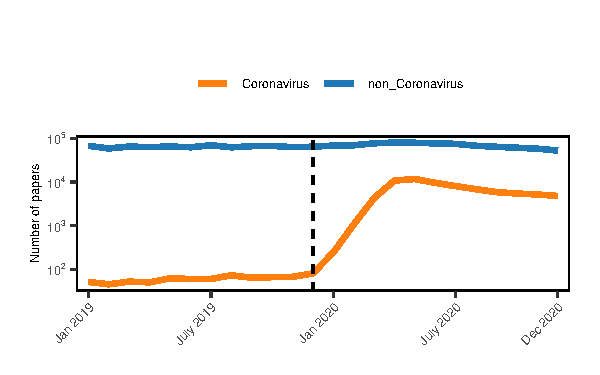
\includegraphics[width=0.7\textwidth]{1_chapter1/figures/Fig1.pdf} %
\caption{\bf Coronavirus and non-coronavirus papers by submission month (log-scale).}
\label{figure1} 
\end{figure*}

Research output in CRR is extremely dynamic, in particular in spring 2020, while it is relatively stable in non-CRR over the analysis period (see Fig~\ref{figure1}). In the pre-COVID-19 period, CRR output is relatively stable, at roughly 50 papers per month. Starting  with the January 2020 outbreak, CRR grows exponentially up to about 11,700 submissions in May 2020 and then decreases again to about 5,000 submissions in December 2020. Non-CRR output is stable throughout, at about 67,000 papers, and even increases slightly with the pandemic.\footnote{Looking closely, one sees non-CRR output decreasing slightly by the end of 2020. For interpretation recall that from October 2020 on the PubMed sample underreports increasingly submissions due to a time lag from submission to publication in PubMed (see Appendix~\ref{sec:AppendixSample}). Therefore, the slight drop of submissions in autumn 2020 (in our sample) does not necessarily indicate potentially negative effects of the pandemic due to frictions in the research machinery, or crowding out of non-coronavirus research. Quantification of such effects must be left to future studies.} \\

The distribution of national health science output is highly skewed, with a Gini coefficient of around 0.9 before and during the pandemic in non-CRR and CRR.\footnote{Gini coefficients are for CRR pre-pandemic 0.90, CRR pandemic 0.87, non-CRR pre-pandemic 0.88, non-CRR pandemic 0.88.} The ten most prolific countries in CRR generate 65 percent of output during COVID-19. In the order of CRR output the top ten countries are (CRR papers in 2019; CRR papers in 2020): USA (225; 21,902), China (192; 9,942), Italy (17; 7,730), UK (54; 6,289),  India (12; 5,260), Spain (14; 3,122), Canada (34; 3,037), Germany (38; 2,931), France (23; 2,923), Australia (29; 2474). All these countries contributed considerably to CRR during the pandemic, but not consistently to CRR before the pandemic. Some scholars explained the (early) high CRR output of China and Italy by the global infection process. On the other hand, rankings based on CRR during the pandemic (in Fig~\ref{figure1}B) correspond surprisingly well to rankings based on overall scientific production in the last two decades (see Table~\ref{tab:WorldScienceOutput}); supporting the idea of the relevance of (slowly-accumulating) science capacity discussed in the `Background' section. 

National scientific output is closely related to IRC also in our sample. Around one fourth of the papers in our sample are internationally co-authored. This holds true for CRR as well as non-CRR papers, before as well as during the pandemic (see Appendix~\ref{sec:AppendixSample}, Table~\ref{tab:DescriptivesSciProd}). Thus, CRR papers during the pandemic are, on average, as international as other papers. 

Looking at the country-level, our data confirms a strong positive relationship between national scientific output and national IRC intensity. In a simple OLS regression of number of internationally co-authored papers on total number of papers (both in logs), we obtain an elasticity of 0.9 for (any) health science papers in 2019, (any) health science papers in 2020, and also for CRR papers in 2020. This exceeds well the estimate of elasticity of 0.7 by \citep{davidson1979international,luukkonen1992understanding}, but seems reasonable if one takes into account the positive trends in IRC observed by \cite{adams2013fourth}. Elasticity for CRR papers in 2019 is slightly lower; around 0.8. Thus IRC may have become somewhat more relevant to national output of CRR during the pandemic, but neither more or less as would be expected on IRC in non-CRR. 

We create international science networks for CRR as well as non-CRR research for each month, from January 2019 to December 2020. Networks are weighted following a full-count assignment, i.e. we increment the weight of the edge between two countries for each paper where both countries appear in the affiliations. Networks are accumulated over time by adding up all edge weights from the beginning of the analysis, January 2019, up to the focal month. Table~\ref{tab:AccumulatedNetworks} provides basic statistics on the accumulating networks. 

In total, we identify 203 countries in our paper affiliations. We aggregate the 2019 period to indicate international scientific activity before the pandemic. At the end of 2019, the (accumulated) CRR network includes 68 countries, with about 500 international co-author ties (edge weights). The accumulated non-CRR network includes in Dec. 2019 nearly all countries, 201, connected through 585k ties. The non-CRR network is stable in 2020. Its decreasing growth rate of IRC papers (Weight \% growth) is due to the addition of a relatively constant number of around 67k IRC papers each month.

Looking at CRR network growth in Table \ref{tab:AccumulatedNetworks}, one may distinguish four phases during which the CRR network expands in 2020. The first month, January 2020, may be considered a first phase in which the CRR network grows mostly in terms of joint papers (edge weights) and less in terms of collaborating countries entering the network (nodes). The second phase, from February to April 2020, is characterized by high growth in terms of both network entrants, around 30 percent growth rate, and joint collaborations, 130 to 300 percent. In the third phase, from May to July 2020, network entry slows down considerably. The growth rate of joint collaborations is very high at the beginning of the phase but slows down during this period from 68 to 22 percent. In a fourth phase, from August to December 2020, few latecomers enter the network and collaboration growth rates stabilize at around ten percent growth per month.  


% latex table generated in R 3.6.3 by xtable 1.8-4 package
% Thu Jul  1 11:10:33 2021
\begin{table}[ht]
\caption{International science networks, CRR and non-CRR, accumulated over months.}
\label{tab:AccumulatedNetworks}
\centering
\begin{tabular}{lrrrrrrrrrrrr}
  \hline
 \multicolumn{13}{l}{\textit{CRR network (accumulated), 2019}} \\
& {\bf Jan.} & {\bf Feb.} & {\bf Mar.} & {\bf Apr.} &  {\bf May} &  {\bf June} &  {\bf July} &   {\bf Aug.} &  {\bf Sept.} &  {\bf Oct.} &  {\bf Nov.} &  {\bf Dec.} \\ Countries & 18 & 26 & 29 & 34 & 40 & 45 & 54 & 54 & 59 & 61 & 66 & 68 \\ 
 Country \% growth &  & 44 & 12 & 17 & 18 & 12 & 20 & 0 & 9 & 3 & 8 & 3 \\ 
 Edge weights & 23 & 39 & 75 & 97 & 123 & 146 & 240 & 266 & 307 & 381 & 427 & 494 \\ 
  Weight \% growth &  & 70 & 92 & 29 & 27 & 19 & 64 & 11 & 15 & 24 & 12 & 16 \\ 
   \hline
 \hline
  \multicolumn{13}{l}{\textit{non-CRR network (accumulated), 2019}} \\
& {\bf Jan.} & {\bf Feb.} & {\bf Mar.} & {\bf Apr.} &  {\bf May} &  {\bf June} &  {\bf July} &   {\bf Aug.} &  {\bf Sept.} &  {\bf Oct.} &  {\bf Nov.} &  {\bf Dec.} \\   \hline
Countries & 188 & 194 & 194 & 198 & 198 & 200 & 201 & 201 & 201 & 201 & 201 & 201 \\ 
  Country \% growth &  & 3 & 0 & 2 & 0 & 1 & 0 & 0 & 0 & 0 & 0 & 0 \\ 
  Edge weights  & 49.8k & 93.6k & 147k & 189k & 240k & 286k & 342k & 389k & 438k & 491k & 539k & 585k \\ 
  Weight \% growth &  & 88 & 57 & 29 & 27 & 19 & 20 & 14 & 13 & 12 & 10 & 9 \\ 
   \hline
  \hline
 \multicolumn{13}{l}{\textit{CRR network (accumulated), 2020}} \\
& {\bf Jan.} & {\bf Feb.} & {\bf Mar.} & {\bf Apr.} &  {\bf May} &  {\bf June} &  {\bf July} &   {\bf Aug.} &  {\bf Sept.} &  {\bf Oct.} &  {\bf Nov.} &  {\bf Dec.} \\   \hline
Countries & 72 & 96 & 116 & 151 & 165 & 171 & 174 & 176 & 179 & 180 & 181 & 182 \\ 
  Country \% growth & 6 & 33 & 21 & 30 & 9 & 4 & 2 & 1 & 2 & 1 & 1 & 1 \\ 
  Edge weights & 673 & 1.5k & 6.1k & 17.5k & 29.4k & 40.2k & 48.9k & 55.0k & 60.9k & 67.5k & 73.9k & 79.8k \\ 
  Weight \% growth & 36 & 131 & 295 & 185 & 68 & 37 & 22 & 12 & 11 & 11 & 9 & 8 \\ 
   \hline
  \hline
 \multicolumn{13}{l}{\textit{non-CRR network (accumulated), 2020}} \\
& {\bf Jan.} & {\bf Feb.} & {\bf Mar.} & {\bf Apr.} &  {\bf May} &  {\bf June} &  {\bf July} &   {\bf Aug.} &  {\bf Sept.} &  {\bf Oct.} &  {\bf Nov.} &  {\bf Dec.} \\   \hline
Countries & 201 & 201 & 201 & 201 & 202 & 203 & 203 & 203 & 203 & 203 & 203 & 203 \\ 
  Country \% growth & 0 & 0 & 0 & 0 & 0 & 0 & 0 & 0 & 0 & 0 & 0 & 0 \\ 
  Edge weights  & 635k & 684k & 739k & 795k & 853k & 910k & 966k & 1016k & 1061k & 1109k & 1149k & 1184k \\ 
  Weight \% growth & 9 & 8 & 8 & 8 & 7 & 7 & 6 & 5 & 4 & 5 & 4 & 3 \\ 
   \hline
\end{tabular}
\end{table}


The first two analyses, Analysis 1 and Analysis 2, aim to shed some light on the role of different factors in driving national and inter-national CRR output over the course of the pandemic. Contextual factors are obtained from several supplementary datasets: The national situation during the pandemic is captured through COVID-19 incidences and governmental measures. The COVID-19 Data Repository by the Center for Systems Science and Engineering (CSSE) at Johns Hopkins University provides COVID-19 cases and deaths \citep{dong2020interactive}.\footnote{The data has been downloaded from https://github.com/owid/covid-19-data/ in March 2021.} Social restrictions and international travel restrictions are obtained from \citet[][]{hale2021global}.\footnote{We use the two data files `international-travel-covid.csv' and `stay-at-home-covid.csv'} National economic data is from the `Penn World Table' \citep{feenstra2015next}. Finally, national socio-economic development is proxied by the human development index obtained from the Human Development Report Office of the United Nations (see hdr.undp.org). Not all countries observed in the publication data are included in the supplementary datasets. Due to missing observations, the number of countries reduces from 201 to 156 countries. All the countries dropped from the sample are small, except for Taiwan that is dropped because the UN does not provide statistics for Taiwan separately from China. 

The third analysis, Analysis 3, focuses on how the development of global CRR during the pandemic relates to global non-CRR. That analysis is based only on publication data, and therefore includes all 201 countries.


\subsection{Analysis 1: National scientific output}
\label{subsec:Analysis1}

\subsubsection{Variables}

\paragraph{CRR.} Our dependent variable is the number of CRR papers accumulated from January 2020 to a given month $t'$, which we shorthand by ($c_{i,t'}$). Accumulating output over months seems reasonable because we are ultimately interested in the dynamics of scientific activity --- not submissions. For example, a paper submitted in April 2020 may well rely on research conducted from January 2020 to March 2020, and may have been influenced by events during that period (e.g. by the infection process for which we control; see below). Alternatively, one may consider the outcome variable as a proxy for the formation of national scientific capacity in CRR during the pandemic.

\paragraph{Initial scientific capacity.} Initial scientific capacity is captured by the accumulated number of CRR (non-CRR) papers up to December 2019, denoted $c_{i,t0}$ ($n_{i,t0}$). 

\paragraph{Pandemic context.} The accumulated number of confirmed deaths associated with the coronavirus, $deaths_{i,t'}$, may be interpreted as a proxy for research needs and opportunities. The number of hospitalized cases would be closer to what we have in mind, but is a less reliable statistic. Pandemic policy restrictions may also be constraining but also inciting research. We include the accumulated number of days with requirement not to leave the house (with minimal exceptions), $lock\text{-}down_{i,t'}$, and the number of days with total border closure, $border\text{-}closed_{i,t'}$. 

\paragraph{Socio-economic context.} Population size in 2019 (in Mio.), $pop_{i,t0}$, GDP per capita in 2019, $gdp_{i,t0}$, (expenditure based PPP in 2017 US Dollars), and the human development index in 2019, $hdi_{i,t0}$, serve to control for country size, economic wealth, and state of development respectively.

We take logs (i.e. $\log(x + 1)$) of all variables except for hdi. The pragmatic argument is that our variables are highly skewed to the right. In theory, one may think of CRR paper production akin to a Cobb-Douglas production process, where factors combine multiplicatively. In this case taking logs of all variables generates a linear model.\footnote{One may think of hdi in this case as the exponent of an exponential in the original multiplicative equation.} 

Table~\ref{tab:DescriptivesAnalysis1} provides basic descriptive statistics of the variables used in the analysis on national scientific output. In addition we add a time indicator running from one in January 2020 to twelve in December 2020. Respective correlation coefficients take up the time trend for all accumulated variables, while initial conditions are fixed over time (zero correlation). 

% latex table generated in R 3.6.3 by xtable 1.8-4 package
% Tue Jun 29 21:23:36 2021
\begin{table}[ht]
\caption{Descriptive statistics (Analysis 1)}
\label{tab:DescriptivesAnalysis1}
\centering
\begin{tabular}{lrrrrrrrrrrrr}
  & Mean & Std.Dev. & \multicolumn{10}{c}{Correlation coefficients}  \\ 
 &  &  & 1 & 2 & 3 & 4 & 5 & 6 & 7 & 8 & 9 & 10 \\ 
  \hline
(1) $c_{i,t'}$ & 3.09 & 2.34 & 1.00 & 0.78 & 0.69 & 0.79 & 0.19 & 0.14 & 0.50 & 0.38 & 0.42 & 0.49 \\ 
 (2) $n_{i,t0}$ & 6.36 & 2.28 & 0.78 & 1.00 & 0.84 & 0.46 & -0.00 & -0.23 & 0.60 & 0.52 & 0.57 & 0.00 \\ 
 (3) $c_{i,t0}$ & 0.82 & 1.17 & 0.69 & 0.84 & 1.00 & 0.38 & -0.00 & -0.22 & 0.55 & 0.43 & 0.46 & 0.00 \\ 
 (4) $deaths_{i,t'}$ & 4.31 & 3.31 & 0.79 & 0.46 & 0.38 & 1.00 & 0.29 & 0.35 & 0.40 & 0.22 & 0.26 & 0.64 \\ 
 (5) $lock\text{-}down_{i,t'}$ & 0.75 & 1.49 & 0.19 & -0.00 & -0.00 & 0.29 & 1.00 & 0.31 & 0.10 & -0.00 & -0.00 & 0.24 \\ 
 (6) $border\text{-}closed_{i,t'}$ & 2.80 & 2.17 & 0.14 & -0.23 & -0.22 & 0.35 & 0.31 & 1.00 & -0.07 & -0.16 & -0.17 & 0.55 \\ 
 (7) $pop_{i,t0}$ & 2.65 & 1.42 & 0.50 & 0.60 & 0.55 & 0.40 & 0.10 & -0.07 & 1.00 & -0.18 & -0.14 & 0.00 \\ 
 (8) $gdp_{i,t0}$ & 9.39 & 1.23 & 0.38 & 0.52 & 0.43 & 0.22 & -0.00 & -0.16 & -0.18 & 1.00 & 0.93 & 0.00 \\ 
 (9) $hdi_{i,t0}$ & 0.73 & 0.15 & 0.42 & 0.57 & 0.46 & 0.26 & -0.00 & -0.17 & -0.14 & 0.93 & 1.00 & 0.00 \\ 
  (10) t & 6.50 & 3.45 & 0.49 & 0.00 & 0.00 & 0.64 & 0.24 & 0.55 & 0.00 & 0.00 & 0.00 & 1.00 \\ 
   \hline
\end{tabular}
\end{table}


\subsubsection{Empirical model}

The estimating equation is the following linear model:

\begin{align*}
c_{i,t'}  = & \beta_{0,t'} + \beta_{1,t'} \: n_{i,t0} + \beta_{2,t'} \: c_{i,t0} + \\ 
 & \beta_{3,t'} \: deaths_{i,t'} + \beta_{4,t'} \: lock\text{-}down_{i,t'} + \beta_{5,t'} \: border\text{-}closed_{i,t'} + \\
 & \beta_{6,t'} \: pop_{i,t0} + \beta_{7,t'} \: gdp_{i,t0} +  \beta_{8,t'} \: hdi_{i,t0} + \epsilon_{i,t'}
\end{align*}

where the $\epsilon_{i,t'}$ denotes the error term. The model is estimated with simple OLS separately for each month $t'$ in 2020. This allows for varying coefficients over time to uncover dynamics. Time effects common to all countries, as for example augmenting number of papers on open source platforms, are then naturally accounted for. For ease of interpretation, all variables are standardized (after taking logs) separately for each month $t'$ to zero mean and standard deviation of one.


\subsection{Analysis 2: International research collaboration}
\label{subsec:Analysis2}

\subsubsection{Variables}

Analysis 2 focusses on drivers of bi-national collaboration on CRR. Some variables describe a single country $i$ (or $j$) that is part of the dyad, others characterize the dyad $ij$. Variables measured before the shock form the initial conditions and are indicated by a time subscript $t0$. Variables that vary over the period of the pandemic are all accumulated over the pandemic (indicated by $t'$). The reason, again, is that a mapping from research context to research output within each month is less likely than a mapping of past and current research context to past and current research output. 

\paragraph{Joint CRR.} The dependent variable is the number of CRR papers signed by two countries $i$ and $j$ between January 2020 up to a given month $t'$, denoted $c_{ij,t'}$. 

\paragraph{Initial scientific capacity.} The number of joint publications in 2019 between both countries on CRR ($c_{ij,t0}$) and non-CRR ($n_{ij,t0}$) are part of initial conditions. For each country, say $i$, we indicate scientific capacity by the total number of CRR papers ($c_{i,t0}$) and non-CRR papers ($n_{i,t0}$). In the link formation context these measures may be interpreted as factors that help to attract or initiate collaborations. In addition, the combination of health science competence is indicated by the sum ($n_{i,t0} + n_{j,t0}$) and absolute difference ($|n_{i,t0} - n_{j,t0}|$). These two factors indicate whether pooled health science capacity in the dyad is high ($n_{i,t0} + n_{j,t0}$) and to what extent scientific capacity is equally distributed among the partners ($|n_{i,t0} - n_{j,t0}|$).

\paragraph{Pandemic context.} The relative pandemic situation of both countries is indicated by taking into account the (accumulated) number of COVID-19 related deaths ($death_{i,t'}$),  number of days under lock-down ($locked_{i,t'}$), and number of days with closed borders ($closed_{i,t'}$). Lock-down and closed borders of a country may hinder initiation or maintenance of international collaboration. Therefore, we keep these variables as individual factors. The number of deaths approximate the number of COVID-19 cases in the country on which research may be conducted. Therefore, we sum cases over the dyad ($death_i + death_j$), and take into account their absolute difference $|death_i - death_j|$. If for example the sum is positively correlated with joint CRR, while the absolute difference is negatively correlated with CRR, then countries with few cases would interact with countries having many cases. Potential explanations for such an observation could be international solidarity but also resource interdependence. 

 
\paragraph{Socio-economic context.} We control for country size by the number of inhabitants in 2019 $pop_{i,t0}$. Economic wealth and development is indicated by gdp per captita ($gdp_{i,t0}$) and the Human Development Index ($hdi_{i,t0}$) respectively. The discussion on core-periphery processes creates an interest in understanding to what extent developed (developing) countries interact among and with each other. Again, the sum and absolute difference of the partners' characteristics provide some indication; leading to the four composite variables $gdp_i + gdp_j$, $|gdp_i - gdp_j|$, $hdi_i + hdi_j$, $|hdi_i - hdi_j|$.


\paragraph{Geographical space.} The literature is clear in that there is a geographical bias in IRC link formation (see Section Background above). Therefore we control for the geographic distance between two countries, $distance_{ij}$, measured by the distance (in km) of the countries' geographic centers. Another control \textit{same\_region}$_{ij}$ indicates whether two countries are located in the same world region, i.e. continent as defined by the World Bank Development Indicators.   



\begin{landscape}
  % latex table generated in R 3.6.3 by xtable 1.8-4 package
% Wed Jun 30 12:09:46 2021
\begin{table}[ht]
	\begin{threeparttable}
\caption{Descriptive statistics (Analysis 2)}
\label{tab:DescriptivesAnalysis2}
\begin{small}
\centering
\begin{tabular}{lrrrrrrrrrrr}
\hline\noalign{\smallskip}
    & Mean & Std.Dev. & \multicolumn{9}{c}{Correlation coefficients}  \\ 
\noalign{\smallskip}\hline\noalign{\smallskip}
		&		&		&	(1)	&	(2)	&	(3)	&	(4)	&	(5)	&	(6)	&	(7)	&	(8)	&	(9)	\\
\noalign{\smallskip}\hline\noalign{\smallskip}
(1)	$c_{ij,t'}$	&	0.46	&	0.93	&	1	&	0.4	&	0.76	&	0.61	&	0.64	&	0.49	&	0.39	&	0.45	&	0.43	\\
(2)	$c_{ij,t0}$	&	0.02	&	0.15	&	0.4	&	1	&	0.35	&	0.35	&	0.27	&	0.2	&	0.16	&	0.11	&	0.11	\\
(3)	$n_{i,t0}$	&	1.54	&	1.72	&	0.76	&	0.35	&	1	&	0.71	&	0.83	&	0.66	&	0.54	&	0.35	&	0.34	\\
(4)	$c_{i,t0}$	&	1.64	&	1.65	&	0.61	&	0.35	&	0.71	&	1	&	0.84	&	0.86	&	0.78	&	0.38	&	0.39	\\
(5)	$n_{i,t0}$	&	12.71	&	3.22	&	0.64	&	0.27	&	0.83	&	0.84	&	1	&	0.91	&	0.8	&	0.43	&	0.43	\\
(6)	$n_{i,t0}+n_{j,t0}$	&	7.84	&	1.92	&	0.49	&	0.2	&	0.66	&	0.86	&	0.91	&	1	&	0.95	&	0.46	&	0.47	\\
(7)	$|n_{i,t0}-n_{j,t0}|$	&	7.31	&	2.3	&	0.39	&	0.16	&	0.54	&	0.78	&	0.8	&	0.95	&	1	&	0.43	&	0.44	\\
(8)	$death_i+death_j$	&	6.19	&	3.15	&	0.45	&	0.11	&	0.35	&	0.38	&	0.43	&	0.46	&	0.43	&	1	&	0.98	\\
(9)	$|death_i-death_j|$	&	5.8	&	3.22	&	0.43	&	0.11	&	0.34	&	0.39	&	0.43	&	0.47	&	0.44	&	0.98	&	1	\\
(10)	$closed_{i,t'}$	&	6.12	&	3.36	&	-0.02	&	-0.09	&	-0.18	&	-0.22	&	-0.22	&	-0.23	&	-0.2	&	0.41	&	0.37	\\
(11)	$locked_{i,t'}$	&	1.64	&	2.22	&	0.08	&	-0.01	&	0.01	&	0	&	0	&	0	&	0	&	0.3	&	0.28	\\
(12)	$pop_{i,t0}$	&	5.29	&	2	&	0.41	&	0.18	&	0.48	&	0.55	&	0.6	&	0.56	&	0.49	&	0.37	&	0.37	\\
(13)	$gdp_i+gdp_j$	&	10.39	&	0.85	&	0.28	&	0.11	&	0.38	&	0.44	&	0.51	&	0.51	&	0.47	&	0.2	&	0.2	\\
(14)	$|gdp_i-gdp_j|$	&	9.44	&	1.34	&	0.05	&	0	&	0.08	&	0.25	&	0.27	&	0.32	&	0.31	&	0.1	&	0.1	\\
(15)	$hdi_i+hdi_j$	&	1.46	&	0.22	&	0.37	&	0.15	&	0.51	&	0.46	&	0.57	&	0.53	&	0.47	&	0.24	&	0.24	\\
(16)	$|hdi_i-hdi_j|$	&	0.18	&	0.13	&	-0.19	&	-0.08	&	-0.24	&	0.02	&	-0.02	&	0.09	&	0.12	&	-0.02	&	-0.01	\\
(17)	distance	&	8.67	&	0.77	&	-0.16	&	-0.07	&	-0.23	&	0.03	&	-0.04	&	0.01	&	0.03	&	0.01	&	0.03	\\
(18)	sameRegion	&	0.24	&	0.43	&	0.16	&	0.06	&	0.2	&	-0.02	&	-0.02	&	-0.06	&	-0.07	&	-0.04	&	-0.05	\\
(19)	t	&	7	&	3.16	&	0.22	&	0	&	0	&	0	&	0	&	0	&	0	&	0.65	&	0.6	\\
\noalign{\smallskip}\hline\noalign{\smallskip}
   & \multicolumn{9}{c}{Correlation coefficients}  \\ 
\noalign{\smallskip}\hline\noalign{\smallskip}
		&	(10)	&	(11)	&	(12)	&	(13)	&	(14)	&	(15)	&	(16)	&	(17)	&	(18)	&	(19)	\\
(1)	$c_{ij,t'}$	&	-0.02	&	0.08	&	0.41	&	0.28	&	0.05	&	0.37	&	-0.19	&	-0.16	&	0.16	&	0.22	\\
(2)	$c_{ij,t0}$	&	-0.09	&	-0.01	&	0.18	&	0.11	&	0	&	0.15	&	-0.08	&	-0.07	&	0.06	&	0	\\
(3)	$n_{i,t0}$	&	-0.18	&	0.01	&	0.48	&	0.38	&	0.08	&	0.51	&	-0.24	&	-0.23	&	0.2	&	0	\\
(4)	$c_{i,t0}$	&	-0.22	&	0	&	0.55	&	0.44	&	0.25	&	0.46	&	0.02	&	0.03	&	-0.02	&	0	\\
(5)	$n_{i,t0}$	&	-0.22	&	0	&	0.6	&	0.51	&	0.27	&	0.57	&	-0.02	&	-0.04	&	-0.02	&	0	\\
(6)	$n_{i,t0}+n_{j,t0}$	&	-0.23	&	0	&	0.56	&	0.51	&	0.32	&	0.53	&	0.09	&	0.01	&	-0.06	&	0	\\
(7)	$|n_{i,t0}-n_{j,t0}|$	&	-0.2	&	0	&	0.49	&	0.47	&	0.31	&	0.47	&	0.12	&	0.03	&	-0.07	&	0	\\
(8)	$death_i+death_j$	&	0.41	&	0.3	&	0.37	&	0.2	&	0.1	&	0.24	&	-0.02	&	0.01	&	-0.04	&	0.65	\\
(9)	$|death_i-death_j|$	&	0.37	&	0.28	&	0.37	&	0.2	&	0.1	&	0.24	&	-0.01	&	0.03	&	-0.05	&	0.6	\\
(10)	$closed_{i,t'}$	&	1	&	0.34	&	-0.07	&	-0.19	&	-0.14	&	-0.17	&	-0.06	&	0.04	&	0	&	0.55	\\
(11)	$locked_{i,t'}$	&	0.34	&	1	&	0.1	&	-0.06	&	-0.09	&	0	&	-0.13	&	0.07	&	0	&	0.27	\\
(12)	$pop_{i,t0}$	&	-0.07	&	0.1	&	1	&	-0.18	&	-0.11	&	-0.14	&	0.04	&	0.05	&	0.03	&	0	\\
(13)	$gdp_i+gdp_j$	&	-0.19	&	-0.06	&	-0.18	&	1	&	0.68	&	0.87	&	0.11	&	-0.01	&	-0.14	&	0	\\
(14)	$|gdp_i-gdp_j|$	&	-0.14	&	-0.09	&	-0.11	&	0.68	&	1	&	0.43	&	0.54	&	0.08	&	-0.22	&	0	\\
(15)	$hdi_i+hdi_j$	&	-0.17	&	0	&	-0.14	&	0.87	&	0.43	&	1	&	-0.25	&	-0.02	&	-0.07	&	0	\\
(16)	$|hdi_i-hdi_j|$	&	-0.06	&	-0.13	&	0.04	&	0.11	&	0.54	&	-0.25	&	1	&	0.13	&	-0.3	&	0	\\
(17)	distance	&	0.04	&	0.07	&	0.05	&	-0.01	&	0.08	&	-0.02	&	0.13	&	1	&	-0.63	&	0	\\
(18)	sameRegion	&	0	&	0	&	0.03	&	-0.14	&	-0.22	&	-0.07	&	-0.3	&	-0.63	&	1	&	0	\\
(19)	t	&	0.55	&	0.27	&	0	&	0	&	0	&	0	&	0	&	0	&	0	&	1	\\
\noalign{\smallskip}\hline
\end{tabular}
\end{small}
	\end{threeparttable}
\end{table}

\end{landscape}



\subsubsection{Empirical model}

The empirical model is essentially a gravity model, where the interaction intensity between two countries (here number of joint CRR papers) depends on the countries' distance and further (relational) factors. The model is common in spatial scientometrics \citep{frenken2009spatial} and has been applied in the same form e.g. by \cite{hoekman2009geography}.

In detail, we estimate a zero-inflated negative binomial model in order to take into account the fact that many (mostly small and distant) countries do not have any joint CRR paper. The model combines the negative binomial count density\footnote{The choice of the negative binomial density over a Poisson density is supported by a strong and significant estimate of the variance related parameter.} with a binary process\footnote{We chose a logit model.} to model excess zeros in the outcome \citep[see e.g.][p.681]{cameron2005microeconometrics}. 

The first part of the model, termed the zero-model, models the binary process of two countries $i$ and $j$ having \textit{no} joint CRR papers. The linear predictor of the zero-model includes the typical ingredients of a gravity model:

\begin{gather+}[1]
	p = Pr\left[ c_{ij,t} = 0 | \boldsymbol{\gamma} \right] = \text{logit}( \gamma_0 + \gamma_1 \log(n_{i,t0} + n_{j,t0}) + \\
	\gamma_2 \log(| n_{i,t0} - n_{j,t0} | ) +
	\gamma_3 \log(distance_{ij}) + \gamma_4 \textit{same\_region}_{ij}  ) \textit{   ,}
\end{gather+}

where ($n_{i,t0}+n_{j,t0}$) captures the joint weight of the two countries in `health sciences', and ($| n_{i,t0} - n_{j,t0} |$) their absolute difference. Geographical proximity is captured by $\textit{distance}_{ij}$ and the $\textit{same region}_{ij}$ dummy. 

With probability $(1-p)$ the count density applies with expectation

\begin{gather+}[1]
	E\left[ c_{ij,t} | \boldsymbol{\beta} \right] = \exp(\beta_0) c_{ij,t0}^{\beta_1} n_{ij,t0}^{\beta_2} (c_{i,t0} c_{j,t0})^{\beta_3} \times \\
	(\textit{d}_{i,t} + \textit{d}_{j,t})^{\beta_4} \left( | \textit{d}_{i,t} - \textit{d}_{j,t} | \right)^{\beta_5} 
	(\textit{gdp}_{i,t0} + \textit{gdp}_{j,t0})^{\beta_6}  \times \\
	\left( | \textit{gdp}_{i,t0} - \textit{gdp}_{j,t0} |  \right)^{\beta_7} 
	(\textit{hdi}_{i,t0} + \textit{hdi}_{j,t0})^{\beta_8} 
	\left( | \textit{hdi}_{i,t0} - \textit{hdi}_{j,t0} | \right)^{\beta_9} \\
	\textit{distance}_{ij}^{\beta_{10}} \: \textit{same\_region}_{ij}^{\beta_{11}} \textit{   ,}
\end{gather+}

where $\exp(\beta_0)$ is a scaling factor (the intercept). Individual variables are introduced above but some notes on the model structure are in order. First, the model allows for a lasting impact of an established relation in non-CRR and CRR through ($n_{ij,t0}$, $c_{ij,t0}$). Second, countries may `attract' IRC through their research competences ($n_{i,t0}$,$c_{i,t0}$). Because this effect is symmetric (the relationship $ij$ is the same as $ji$), we enforce the same coefficient for $i$ and $j$. Control variables are entered such that they capture the joint `mass' of the partners as well as their absolute difference. For example scientific interaction may be driven by countries having many COVID-19 cases in sum $(\textit{d}_{i,t} + \textit{d}_{j,t})$, but also if one country has many more cases than the other $(| \textit{d}_{i,t} - \textit{d}_{j,t} |)$. The former can be interpreted as a common pool of resources (or incentives), the second captures dyadic interdependence due to inequality in resources.\footnote{We tried various ways of introducing country specific factors into the model, and found this formulation to be the most compelling (in terms of fit and reasoning).} Third, we introduce geographic distance and same region indicators in the count model because geographic proximity is susceptible of driving not only whether but also how much research is conducted jointly. 

The zero-model is kept relatively light, in form of a basic gravity model, for the following reasoning. First, one may interpret the zero-model as the potential to collaborate in the health sciences as such. This is mostly an issue of mutual (or one-sided) awareness driven by a combination of global visibility and geographic distance. Given awareness, the intensity of joint CRR may then be determined by various factors capturing the needs and benefits of collaboration. There is also a more pragmatic argument. The two-step process is an artificial interpretation of the model. In fact, we deal here with one convolution of densities that is determined by all the factors that we consider at once. In this sense, separating factors in the different parts helps to clarify the overall contribution of individual factors to the outcome.  

The link formation model is estimated on dyadic data which by construction may result in network correlation of errors. In general, correlated errors maintain unbiasedness and consistency of coefficient estimates, but create a downward bias of the estimated standard deviations of coefficient estimates. The reason is essentially that (network) dependence of observations reduces the information content compared to independent observations (which is assumed by standard estimators). Most of the dependence across dyad observations can be expected from repeated observations for the same individual countries. The Multiple Regression Quadratic Assignment Procedure (MRQAP) therefore creates a Null distribution through random permutation of rows and columns of the adjacency matrix (in effect a random re-labeling of nodes in the network). In principle, there are different ways to implement the idea of MRQAP (Decker et al., 2007). In our case, the preferred choice is to permute one right-hand-side factor, keeping everything else fixed, to generate the distribution of the z-statistic (coefficient estimate divided by its standard deviation) under the Null hypothesis that the right-hand-side factor is not systematically related to the outcome controlling for all other factors.\footnote{There are pros and cons to the different ways of implementing MRQAP. The simplest way would be to permute the outcome but that has the disadvantage to create a distribution under the null that no factor is relevant. Furthermore, our (non-linear) model fails to converge if the model does not fit the data, which is almost always the case when the outcome is permuted. Permutation of error terms after partialing is a common alternative but is only valid under relatively strict assumptions on the error term which are unlikely to be met in our model as it is a convolution of two different distributions. Our preferred alternative of permuting individual right hand side factors has the disadvantage to break existing correlation with other right hand side factors. The effect seems however to be bearable if a pivotal statistic is used, as we do \citep{dekker2007sensitivity}.} In the results, we report the estimated z-value together with significance levels of one-sided tests based on the Null distribution of z-values from permutation.  

%We turn now to the question which factors are correlated with the intensity of CRR between two countries during the pandemic. Fig~\ref{figure1}D provides a first descriptive indication. The surface plot is obtained from a local regression with least-squares cross-validated bandwidths for the local constant estimator. It shows the expected (log of) joint coronavirus papers during COVID-19, conditional on (log of) joint coronavirus and non-coronavirus papers pre-COVID-19. Most country-pairs (dots) had no pre-COVID-19 joint coronavirus research. Their number of joint coronavirus papers during COVID-19 increases with the number of other joint papers before the pandemic. As we increase from zero prior coronavirus papers, (expected) joint coronavirus papers during COVID-19 (the surface in Fig~\ref{figure1}D) also increases. Yet, it is evident that bi-national collaboration on coronavirus related research after the shock largely reflects bi-national collaboration on non-coronavirus research before the shock. 


\subsection{Analysis 3: Convergence to global health science}
\label{subsec:Analysis3}

The COVID-19 shock changed dramatically the global distribution of CRR.  Because the global health science system responded in very short time, CRR during the pandemic must have built essentially on resources developed before the outbreak. Therefore it seems reasonable that the global structure of CRR during the pandemic converges to the (pre-pandemic) global structure of health sciences. We investigate this hypothesis by looking at i) national scientific output, ii) countries' network centrality in the IRC network, and iii) IRC network structure. 

\subsubsection{National scientific output}

For each month in 2019 and 2020, we create a ranking of countries based on CRR output ($c_{i,t}$) and non-CRR output ($n_{i,t}$) respectively. We speak of convergence in national scientific output when the two rankings become more similar over time. Similarity is appropriately captured by the rank correlation coefficient $\tau_X$, as described in \cite{emond2002new}. This statistic is similar to Kendall's $\tau$, except that it handles ties the same as dominant relationships (entering 1 and not 0 in the dominance matrix). In principle, this is favorable in case of many ties in the rankings, as we have in corona pre-Covid-19 research; but does not really effect the results. A 90 percent confidence interval around $\tau_X$ is then obtained by a traditional jackknife, or leave-one-out, approach as described for example in \cite{abdi2010jackknife}.

\subsubsection{Network centrality}

The international science network is highly hierarchical, and network centrality captures the position of a country within that hierarchy. Therefore, we ask `How does network centrality of countries in the CRR network align with their centrality in the overall health science network?'

Although one may argue on the details, the international science network can be safely said to exhibit a core-periphery structure. Therefore, network centrality is appropriately captured through (normalized) s-core decomposition \citep{eidsaa2013s}. The s-core decomposition identifies sets of nodes that are heavily connected among each other. Together they form the network core(s). Roughly, the algorithm starts from the complete network and proceeds by iterative removal of the least connected node in the remaining network. The s-core is the strength of the node in the (remaining) network at the time of removal. In order to compare different networks over time, we normalize the s-core by the maximum s-core in the network. The s-core ranges from 0 for isolates in the network, to 1 for (highest) core members. S-cores are measured for each country on a monthly bases on the CRR network and the non-CRR network respectively. As the difference between the s-cores decreases, hierarchies converge. 

\subsubsection{Network structure}

Convergence in network structure is first investigated by correlating the CRR adjacency matrix with the non-CRR adjacency matrix on a monthly basis. The weights in the adjacency matrix are in logs because they are highly skewed --- many countries do not collaborate (zero entry) and some do heavily (many joint papers). Statistical significance of correlations is obtained through the Quadratic Assignment Procedure (QAP). The QAP test creates a null distribution through re-labeling of nodes in one network; maintaining the structure of the networks. The correlation analysis tells us whether the CRR network and the non-CRR network become more similar over time.  

In a second step, we investigate in which aspects the CRR network differs from the non-CRR network. The background section highlights network hierarchy and communities as two salient features in ICR networks. This is what we focus on. 

Hierarchy is captured by the largest (absolute) eigenvalue of the adjacency matrix, say $\lambda$. More hierarchical networks tend to have a higher largest eigenvalue. In fact, it has been shown that the largest eigenvalue is maximal for nested-split graphs. A nested-split graph is a specific type of a hierarchical network, in which the most central node connects to all other nodes, and less central nodes connect to subsets of alters of more central nodes. Interestingly, nested-split graphs emerge in network games where payoffs are strategic complements in effort levels \citep{konig2014nestedness}, which is a reasonable assumption for science networks. 

We measure $\lambda$ on the (accumulating) CRR network for each month from January 2019 to December 2020. The value of $\lambda$ in itself is not very telling as it depends on various features of the network; most importantly network size. For interpretation it is therefore useful to compare this statistic to a network null model in order to see whether the network of interest is more or less hierarchical as the null network. Most studies create a null distribution of networks be fixing some aspects of the focal network, e.g. network size and degree distribution, and randomize the rest. Our interest is in how the CRR network structurally deviates from the non-CRR network. Therefore we use the non-CRR network formed in 2019 to generate our null distribution. In detail, one realization $s$ is obtained by drawing links uniformly at random with replacement from the non-CRR network until a network is created of the same size (same number of links, and hence same total strength) as the CRR network. Each realization yields a statistic $\lambda_s$. We draw 100 realizations to obtain the null distribution for our statistics. Based on the null distribution, we calculate the $z$-value for the largest eigenvalue $\lambda$, as $z_\lambda = \frac{\lambda_{crr} - \hat{E}\left[ \lambda_s \right]}{\widehat{sd}(\lambda_s)}$. A statistic $z_\lambda$ below (above) zero indicates that the CRR network is more (less) hierarchical than would be expected by the structure of the (prior) non-CRR network. 

Network communities are commonly thought of as subsets of nodes with relatively strong interaction. IRC networks feature communities due to scientists' tendency to collaborate with other scientists that are somewhat close in space; with space broadly defined as scientific, geographical, cultural etc. (see Section Background). The hypothesis we wish to test is that during the pandemic the (accumulating) CRR network converges towards the same community structure as the (prior) non-CRR network. The outline of our empirical approach is as follows: In a first step, we detect communities in the (prior) non-CRR network. This becomes our reference community structure, say benchmark. Then, for each month in the observation period, we measure how well the (accumulating) CRR network `fits' that benchmark. As in the hierarchy analysis, we account for varying network sizes over time and across networks by creating a null distribution through resampling from the non-CRR network. We discuss the details in the following.


Community detection in the (prior) non-CRR network follows closely the procedure of \cite{fitzgerald2021academia}. The main idea is to find a network partition that maximizes some network modularity statistic, say $Q$. \citet{newman2004analysis} proposed a statistic that measures to what extent nodes belonging to the same community form (weighted) ties beyond what would be expected based on their link strength alone.\footnote{In some sense, the null model here is a simple gravity model based on only node size. In the prior IRC literature a similar normalization has been applied by calculating Salton's measure, i.e. observed strength of interaction between two nodes divided by the product of the nodes network strength. Salton's measure revealed in particular country preferences of interaction, revealing the role of distance in IRC.} \cite{reichardt2006statistical} proposed multiple generalizations known as spin-glass algorithm. Among others they introduce a parameter $\gamma$ for tuning the resolution of the network partition. A smaller (higher) $\gamma$ tends to yield less (more) clusters. For $\gamma = 1$ the objective function coincides with Newman's network modularity measure \citep{newman2004analysis}. We use that extension. The optimization is done through simulated annealing (as implemented in the R-package `igraph'). Simulated annealing is a stochastic optimization algorithm and hence may provide different partitions for the same data and parameter settings. This is actually useful, because the robustness of communities for a given parameter $\gamma$ across multiple optimizations signals whether communities are well identified. We search a robust and informative community partitioning through a grid search on $\gamma$. Appendix XY details how. 


\begin{figure*}[!h]
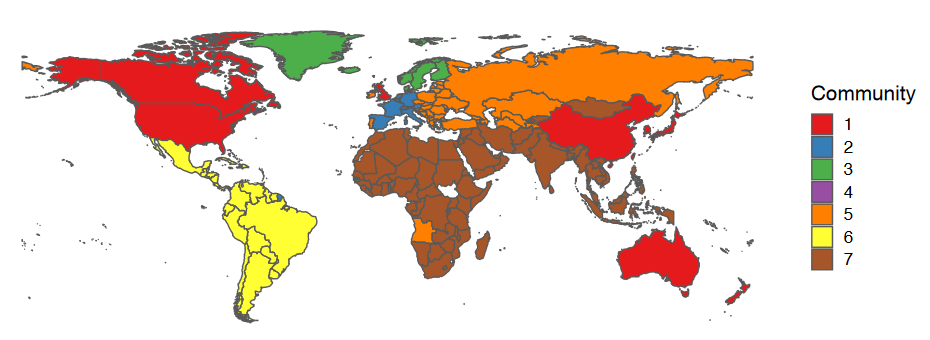
\includegraphics[width=0.9\textwidth]{1_chapter1/figures/Fig2.png} %
\caption{{\bf Communities in the 2019 non-CRR network from spin-glass algorithm with tuning parameter $\gamma=1.2$; the reference community structure for Analysis 3.3.}}
\label{fig:CommWorldmap} 
\end{figure*}

Figure~\ref{fig:CommWorldmap} displays a partition of the (2019) non-CRR network for $\gamma=1.2$. It is remarkable how similar that partitioning is to the partitioning obtained by \citet[][Fig.5b]{fitzgerald2021academia} based on all Scopus publications in 2015. The map displays seven communities with numbers ordered by the average network strength of their members (Appendix \ref{Appendix:Communities} lists the countries belonging to each community). Community 1 is a global community that includes most importantly the US, China, Great Britain, and Japan. All other communities cover world regions. Roughly, Community 2 covers Central Europe, Community 3 Northern Europe, Community 4 includes only Israel, Jersey, and Montserrat, Community 5 spans East Europe and Russia, Community 6 corresponds to South America, and Community 7 covers Africa and the Middle East. 

This partition is used in the analysis as the benchmark for the (accumulating) CRR network. For each month in the observation period, we calculate the modularity statistic on the (accumulating) CRR network ($Q_{crr}$) on the benchmark partitioning obtained in the previous step on the non-CRR network. In addition, multiple resamples are obtained from the non-CRR network such that each resample $s$ has the same size (i.t.o. total edge weights) as the (current) CRR network. As for the CRR network, we calculate for each resample of the non-CRR network a modularity statistic, $Q_s$. This provides us a $z$-value, i.e. $z_Q =  \frac{Q_{crr} - \hat{E}\left[ Q_s \right]}{\widehat{sd}(Q_s)}$. If the $z$-value is high (low) we can say that the CRR network fits well (badly) the community structure of the (2019) non-CRR network. 



\section{Results}


\subsection{National scientific output}
\label{sec:NatSciProd}

Table~\ref{tab:NationalCRR} shows regressions of the cumulative number of national CRR papers for each month in 2020. In the first column, January 2020, pre-pandemic CRR ($c_{t0}$) and the number of COVID-19 related deaths ($deaths_{t'}$) are estimated to be significantly and positively correlated. Other factors appear to be weakly correlated to CRR in January 2020. However, within the first months of the pandemic --- as CRR takes off --- this pattern reverses. More general health science capacity ($n_{t0}$) becomes the dominating factor of CRR output. The relevance of CRR specific experience diminishes gradually, and the impact of (national) COVID-19 cases immediately goes down on a stable and low level. Experiencing a lock down ($locked_{t'}$) tends to be also positively related to output but not very significantly. The discussion above already hints to a potential ambiguity in the effect from lock down experience in that it may signal research needs and opportunities (certainly not fully captured by the number of COVID-19 related deaths), as well as actual constraints to research. Closed international borders (as we measure by $border_{t'}$) seem to have no effect on scientific output. Also population size ($pop_{t0}$) and GDP per capita ($gdp_{t0}$) take over little explanatory power once (prior) research output is controlled for. Finally, the state of economic and social development ($hdi_{t0}$) is negatively correlated with output controlling for confounding factors. Although the estimated coefficient is (mostly) insignificant, there is a clear negative trend, suggesting that in particular in the second half of 2020 less developed countries engaged more in CRR research. Finally, note that model fit in terms of $R^2$ increases from around 0.8 in January to 0.95 in December. This suggests that the factors taken into account in the regression `fit' increasingly well with variations of national CRR.

{\newgeometry{bottom=3cm,asymmetric}
\begin{landscape}
% latex table generated in R 3.6.3 by xtable 1.8-4 package
% Tue Jun 22 10:11:22 2021
\begin{table}
	\begin{threeparttable}
\centering
\caption{Accumulated number of CRR papers ($c_{t'}$) in 2020 (all variables in logs, standardized to zero mean and one std.dev., 156 countries).}
\label{tab:NationalCRR}
\begin{small}
\begin{tabular}{lcccccccccccc}
\hline\noalign{\smallskip}
  & {\bf Jan.} & {\bf Feb.} & {\bf Mar.} & {\bf Apr.} &  {\bf May} &  {\bf June} &  {\bf July} &   {\bf Aug.} &  {\bf Sept.} &  {\bf Oct.} &  {\bf Nov.} &  {\bf Dec.} \\ 
  & {\bf`20}   & {\bf`20}     & {\bf`20}.    & {\bf`20}  & {\bf`20}   & {\bf`20}     & {\bf`20} & {\bf`20} & {\bf`20} & {\bf`20} & {\bf`20} & {\bf`20}  \\
\noalign{\smallskip}\hline\noalign{\smallskip}
   $n_{t0}$ & 0.048   & 0.219 *  & 0.62 ***  & 0.786 ***  & 0.851 ***  & 0.929 ***  & 0.928 ***  & 0.931 ***  & 0.94 ***  & 0.948 ***  & 0.943 ***  & 0.942 ***  \\ 
   & (0.095) & (0.087) & (0.07) & (0.059) & (0.058) & (0.054) & (0.053) & (0.05) & (0.049) & (0.048) & (0.049) & (0.05) \\ 
  $c_{t0}$ & 0.764 ***  & 0.577 ***  & 0.308 ***  & 0.144 ***  & 0.099 *  & 0.063   & 0.066   & 0.05   & 0.044   & 0.035   & 0.029   & 0.025   \\ 
   & (0.071) & (0.066) & (0.051) & (0.041) & (0.041) & (0.038) & (0.038) & (0.036) & (0.035) & (0.035) & (0.036) & (0.036) \\ 
  $deaths_{t'}$ & 0.134 ***  & 0.089   & 0.086   & 0.1 *  & 0.084 *  & 0.08 *  & 0.075 *  & 0.091 **  & 0.095 **  & 0.088 **  & 0.072 *  & 0.062 *  \\ 
   & (0.04) & (0.059) & (0.047) & (0.04) & (0.037) & (0.032) & (0.032) & (0.03) & (0.029) & (0.029) & (0.029) & (0.029) \\ 
  $locked_{t'}$ & --- & 0.023   & 0.022   & 0.049 *  & 0.058 *  & 0.053 *  & 0.06 **  & 0.057 **  & 0.053 **  & 0.052 **  & 0.053 **  & 0.055 **  \\ 
   & --- & (0.055) & (0.028) & (0.023) & (0.023) & (0.021) & (0.021) & (0.02) & (0.02) & (0.02) & (0.02) & (0.02) \\ 
  $border_{t'}$ & --- & --- & 0.013   & 0.01   & -0.013   & -0.006   & -0.004   & -0.006   & -0.003   & -0.004   & -0.007   & -0.01   \\ 
   & --- & --- & (0.028) & (0.023) & (0.024) & (0.022) & (0.022) & (0.022) & (0.021) & (0.021) & (0.021) & (0.021) \\ 
  $pop_{t0}$ & 0.06   & 0.13 *  & 0.021   & -0.019   & -0.026   & -0.048   & -0.044   & -0.041   & -0.039   & -0.033   & -0.011   & 0.001   \\ 
   & (0.07) & (0.064) & (0.053) & (0.045) & (0.046) & (0.044) & (0.045) & (0.042) & (0.041) & (0.041) & (0.041) & (0.041) \\ 
  $gdp_{t0}$ & 0.002   & 0.079   & 0.017   & 0.042   & -0.005   & 0.018   & 0.05   & 0.076   & 0.097   & 0.101   & 0.113 *  & 0.115 *  \\ 
   & (0.103) & (0.095) & (0.075) & (0.061) & (0.062) & (0.058) & (0.057) & (0.054) & (0.052) & (0.052) & (0.052) & (0.053) \\ 
  $hdi_{t0}$ & 0.001   & -0.056   & -0.07   & -0.064   & -0.043   & -0.096   & -0.123 *  & -0.143 *  & -0.167 **  & -0.17 **  & -0.171 **  & -0.168 **  \\ 
   & (0.11) & (0.101) & (0.081) & (0.067) & (0.066) & (0.061) & (0.061) & (0.058) & (0.056) & (0.056) & (0.057) & (0.058) \\ 
\noalign{\smallskip}\hline\noalign{\smallskip}
  $R^2$ & 0.795 & 0.829 & 0.895 & 0.929 & 0.928 & 0.938 & 0.938 & 0.944 & 0.948 & 0.949 & 0.949 & 0.947 \\ 
\noalign{\smallskip}\hline\noalign{\smallskip}
\end{tabular}
  \end{small}
    \begin{tablenotes}
  \footnotesize
  \item {\it Notes:} Recall from Section \ref{subsec:Analysis1} that $c_{t0}$ and $n_{t0}$ proxy initial scientific capacity in CRR and non-CRR respectively. The main finding is that correlation of $c_{t0}$ with CRR output starts off high but decreases as $n_{t0}$ takes over the main explanatory power. There is some support that national pandemic severity ($deaths_{t'}$, $locked_{t'}$) are positively, and economic development ($hdi_{t0}$) is negatively associated with CRR by the second half of 2020.
    \end{tablenotes}
  \end{threeparttable}
\end{table}
\hfill
\end{landscape}}


\subsection{International research collaboration}
\label{sec:IRC}

Estimation results presented in Table~\ref{tab:jointCRR} provide information on the dynamics of joint CRR over the pandemic, taking into account various factors. Regressions of accumulated number of joint CRR papers start in February 2020 and are estimated separately for each month up to December 2020.\footnote{For January 2020, the first month of the pandemic, the outcome variable has been very sparse. Therefore the model did not fit the data and the estimation failed to convergence.} The discussion below focusses on coefficient estimates. Note that coefficient estimates are not to be interpreted as elasticities. Average marginal effects are therefore provided in the Appendix~\ref{sec:MargEffects}, Table~\ref{tab:margEff}. 

Focus on the first column (February 2020). The zero model (lower part of the table) estimates the probability of having \textit{no} joint CRR. The sum of non-CRR papers in 2019 ($n_{i,t0} + n_{j,t0}$) is negative and highly significant, meaning that chances increase to have (at least one) joint CRR paper in 2020. Absolute difference in non-CRR papers make little difference; if anything (as a positive coefficient is estimated) inequality makes it less likely to work together. Geographic distance plays no (significant) role as such, but being in the same region is positively related to joint CRR in February 2020. Looking at the count model of the intensity of dyadic CRR, we estimate a coefficient of one for joint non-CRR in the prior year 2019. Joint CRR papers are positively but not significantly correlated. Once past dyadic interaction is taken into account, countries with large health science capacity ($n_{i,t0}$) are not sought initially. On the other hand, countries with specific CRR capacity attract collaborators ($c_{i,t0}$). The pandemic state of the country, i.e. COVID-19 related deaths, lock-downs, and closed borders, do not play a role initially; probably because too few countries in the sample are hit. Country size (pop) and economic wealth (gdp per capita) play a role initially. There is some sign that developing countries collaborate with each other (negative $hdi_i + hdi_j$), but not particularly with more advanced countries (negative $|hdi_i - hdi_j|$). One percent increases reduce the outcome by 1.9 and 0.5 percent respectively. Geographic distance and being located in the same region are not significant in the count model. The significant technical parameter $\tau$ indicates that the negative binomial model actually does capture over-dispersion.


{\newgeometry{bottom=2cm,asymmetric}
\begin{landscape}

% latex table generated in R 3.6.3 by xtable 1.8-4 package
% Fri Jun 25 12:45:15 2021
\begin{table}[ht]
\begin{threeparttable}
\centering
\caption{Zero-inflated negative binomial model of (accumulated) joint coronavirus related papers  ($c_{ij,t'}$) during the pandemic, est. coefficient (z-value, p-value)}
\label{tab:jointCRR}
\begin{tiny}
\begin{tabular}{rlllllllllll}
\hline\noalign{\smallskip}
    & {\bf Feb. `20} & {\bf Mar. `20} & {\bf Apr. `20} &  {\bf May `20}  &  {\bf June `20} &  {\bf July `20} &  {\bf Aug. `20} &  {\bf Sept. `20} &  {\bf Oct. `20} &  {\bf Nov. `20} &  {\bf Dec. `20}   \\ 
\noalign{\smallskip}\hline\noalign{\smallskip}
       	\textit{Count-model} & & & & & & & & & & & \\
\noalign{\smallskip}
  Intercept & -4.809*** & -8.207*** & -5.198*** & -3.032*** & -3.617*** & -3.919*** & -4.286*** & -4.346*** & -4.178*** & -4.287*** & -4.138*** \\ 
  & (-3.038, 0) & (-10.428, 0) & (-9.735, 0) & (-6.858, 0) & (-9.316, 0) & (-10.698, 0) & (-11.962, 0) & (-12.55, 0) & (-12.322, 0) & (-12.611, 0) & (-12.331, 0) \\ 
$n_{ij,t0}$ & 1.048*** & 0.67*** & 0.809*** & 0.841*** & 0.762*** & 0.722*** & 0.717*** & 0.722*** & 0.728*** & 0.74*** & 0.753*** \\ 
   & (13.816, 0) & (20.086, 0) & (33.21, 0) & (41.296, 0) & (42.372, 0) & (42.162, 0) & (42.554, 0) & (44.636, 0) & (46.044, 0) & (47.304, 0) & (49.144, 0) \\ 
  $c_{ij,t0}$ & 0.174 & 0.044 & 0.005 & 0.005 & 0.053 & 0.059 & 0.057 & 0.034 & 0.025 & 0.028 & 0.025 \\ 
   & (1.69, 0.088) & (0.872, 0.228) & (0.105, 0.419) & (0.125, 0.464) & (1.312, 0.178) & (1.438, 0.177) & (1.376, 0.186) & (0.862, 0.266) & (0.616, 0.302) & (0.667, 0.32) & (0.605, 0.293) \\ 
$n_{i,t0}$ & -0.536*** & 0.262*** & 0.09 & 0.038 & 0.15*** & 0.167*** & 0.173*** & 0.175*** & 0.149*** & 0.148*** & 0.138*** \\ 
   & (-7.028, 0) & (7.028, 0) & (3.599, 0.059) & (1.859, 0.193) & (8.261, 0) & (9.729, 0) & (10.293, 0) & (10.794, 0) & (9.48, 0) & (9.441, 0) & (8.982, 0) \\ 
 $c_{i,t0}$ & 0.301** & 0.019 & 0.04 & 0.049 & -0.003 & 0.005 & 0.007 & 0.022 & 0.032 & 0.015 & 0.017 \\ 
   & (5.151, 0.009) & (0.741, 0.36) & (2.165, 0.196) & (3.161, 0.142) & (-0.203, 0.486) & (0.419, 0.418) & (0.577, 0.431) & (1.814, 0.265) & (2.583, 0.186) & (1.25, 0.337) & (1.403, 0.29) \\ 
  $death_i + death_j$ & -0.943 & 0.023 & 0.067 & 0.059 & 0.062 & 0.096* & 0.108* & 0.131*** & 0.166*** & 0.136*** & 0.134*** \\ 
   & (-1.386, 0.266) & (0.574, 0.411) & (2.532, 0.119) & (2.513, 0.145) & (2.978, 0.115) & (4.927, 0.014) & (5.433, 0.012) & (6.971, 0) & (8.953, 0) & (7.387, 0) & (7.498, 0) \\ 
  $|death_i - death_j|$ & 1.036 & -0.038 & -0.054 & -0.034 & -0.025 & -0.05 & -0.057 & -0.072* & -0.092** & -0.07* & -0.075* \\ 
   & (1.512, 0.201) & (-1.168, 0.313) & (-2.567, 0.133) & (-1.812, 0.226) & (-1.51, 0.262) & (-3.199, 0.093) & (-3.586, 0.074) & (-4.914, 0.012) & (-6.45, 0.002) & (-4.931, 0.023) & (-5.44, 0.02) \\ 
  $locked_{i,t'}$ & -0.059 & 0.035 & 0.029 & 0.024 & 0.019 & 0.03* & 0.024 & 0.022 & 0.024* & 0.019 & 0.02 \\ 
   & (-0.586, 0.315) & (2.252, 0.175) & (3.635, 0.1) & (3.705, 0.082) & (3.405, 0.121) & (5.842, 0.026) & (4.771, 0.059) & (4.665, 0.051) & (5.096, 0.043) & (4.176, 0.087) & (4.475, 0.075) \\ 
  $closed_{i,t'}$ &  & 0.06* & 0.018 & 0.007 & 0.012 & 0.021* & 0.03** & 0.031** & 0.032*** & 0.031** & 0.03*** \\ 
   &  & (4.846, 0.014) & (2.815, 0.105) & (1.301, 0.295) & (2.737, 0.128) & (5.074, 0.017) & (7.135, 0.006) & (7.816, 0.003) & (8.057, 0) & (7.693, 0.002) & (7.681, 0) \\ 
 $pop_{i,t0}$ & 0.239*** & -0.008 & 0.037 & 0.035 & -0.013 & 0.01 & 0.019 & 0.005 & 0.006 & 0.019 & 0.024 \\ 
   & (5.136, 0) & (-0.323, 0.433) & (2.081, 0.177) & (2.26, 0.155) & (-0.91, 0.351) & (0.752, 0.404) & (1.451, 0.31) & (0.383, 0.458) & (0.47, 0.411) & (1.566, 0.268) & (2.013, 0.221) \\ 
$gdp_i + gdp_j$ & 0.671* & 0.415* & 0.164 & 0.074 & 0.225* & 0.229* & 0.309** di& 0.327** & 0.304** & 0.345** & 0.341** \\ 
   & (3.119, 0.014) & (3.827, 0.025) & (2.152, 0.141) & (1.164, 0.302) & (4.073, 0.031) & (4.42, 0.031) & (6.123, 0.003) & (6.707, 0.001) & (6.384, 0.005) & (7.243, 0.002) & (7.262, 0.001) \\ 
  $|gdp_i - gdp_j|$ & 0.059 & 0.029 & 0.049 & 0.05 & 0.047 & 0.043 & 0.04 & 0.042 & 0.038 & 0.034 & 0.036 \\ 
   & (1.17, 0.207) & (1.331, 0.257) & (2.972, 0.084) & (3.361, 0.057) & (3.592, 0.058) & (3.43, 0.075) & (3.212, 0.093) & (3.461, 0.081) & (3.113, 0.112) & (2.785, 0.112) & (3.009, 0.095) \\ 
 $hdi_i + hdi_j$ & -2.703* & -2.78** & -1.216* & -1.16* & -2.183*** & -2.058*** & -2.303*** & -2.403*** & -2.172*** & -2.33*** & -2.322*** \\ 
   & (-3.17, 0.016) & (-5.925, 0.001) & (-3.723, 0.032) & (-4.364, 0.019) & (-9.428, 0) & (-9.459, 0) & (-10.862, 0) & (-11.709, 0) & (-10.83, 0) & (-11.547, 0) & (-11.646, 0) \\ 
 $|hdi_i - hdi_j|$ & -2.23** & -1.627** & -1.882** & -1.585*** & -1.896*** & -1.835*** & -1.95*** & -1.95*** & -1.817*** & -1.898*** & -1.86*** \\ 
   & (-3.217, 0.009) & (-4.633, 0.005) & (-7.404, 0.001) & (-7.509, 0) & (-10.41, 0) & (-10.657, 0) & (-11.525, 0) & (-11.916, 0) & (-11.303, 0) & (-11.83, 0) & (-11.784, 0) \\ 
  distance & 0.17 & 0.042 & 0.036 & 0.031 & 0.011 & -0.015 & -0.039 & -0.042 & -0.038 & -0.029 & -0.022 \\ 
   & (2.094, 0.075) & (1.214, 0.261) & (1.444, 0.264) & (1.442, 0.246) & (0.583, 0.419) & (-0.85, 0.371) & (-2.167, 0.197) & (-2.378, 0.159) & (-2.187, 0.18) & (-1.633, 0.244) & (-1.245, 0.318) \\ 
  same region & 0.137 & 0.166* & 0.062 & 0.092 & 0.095* & 0.124** & 0.12** & 0.146*** & 0.185*** & 0.179*** & 0.19*** \\ 
   & (0.888, 0.206) & (2.541, 0.038) & (1.267, 0.139) & (2.225, 0.05) & (2.598, 0.02) & (3.562, 0.002) & (3.524, 0.004) & (4.421, 0) & (5.659, 0) & (5.451, 0) & (5.836, 0) \\ 
     $log(\theta)$ & 0.785*** & 1.779*** & 1.533*** & 1.425*** & 1.487*** & 1.428*** & 1.382*** & 1.441*** & 1.357*** & 1.288*** & 1.258*** \\ 
  & (3.563, 0) & (13.876, 0) & (19.336, 0) & (21.71, 0) & (24.631, 0) & (26.305, 0) & (26.816, 0) & (28.767, 0) & (28.25, 0) & (27.91, 0) & (28.142, 0) \\ 
   \noalign{\smallskip}\hline\noalign{\smallskip}
      	\textit{Zero-model} & & & & & & & & & & & \\
\noalign{\smallskip}
 Intercept & 9.385** & 22.461*** & 7.433*** & 5.323*** & 6.008*** & 6.051*** & 5.666*** & 6.498*** & 7.372*** & 7.078*** & 7.55*** \\ 
   & (2.271, 0.005) & (3.59, 0) & (3.248, 0) & (3.716, 0) & (4.713, 0) & (4.489, 0) & (4.305, 0) & (4.896, 0) & (5.666, 0) & (5.684, 0) & (6.151, 0) \\ 
 $n_{i,t0} + n_{j,t0}$ & -2.055** & -10.23*** & -3.237** & -2.454** & -2.373*** & -3.092*** & -3.12*** & -3.049*** & -3.68*** & -3.152*** & -3*** \\ 
   & (-4.084, 0.006) & (-2.837, 0) & (-4.034, 0.002) & (-9.751, 0.004) & (-8.829, 0) & (-7.1, 0) & (-7.14, 0) & (-7.329, 0) & (-7.391, 0) & (-8.236, 0) & (-8.991, 0) \\ 
  $|n_{i,t0} - n_{j,t0}|$ & 0.674 & 8.523 & 1.788 & 1.088** & 1.129*** & 1.755* & 1.776** & 1.651** & 2.196** & 1.656** & 1.499** \\ 
  & (1.864, 0.101) & (2.517, 0.088) & (2.355, 0.073) & (4.916, 0.004) & (4.648, 0) & (4.266, 0.0122) & (4.31, 0.009) & (4.245, 0.004) & (4.717, 0.009) & (4.753, 0.004) & (4.992, 0.005) \\ 
  distance & 0.293 & -0.812 & 0.523 & 0.659** & 0.436* & 0.508** & 0.557** & 0.5** & 0.498** & 0.523** & 0.464** \\ 
   & (0.72, 0.314) & (-1.739, 0.079) & (2.067, 0.057) & (4.189, 0.004) & (3.295, 0.012) & (3.604, 0.009) & (4.057, 0.001) & (3.641, 0.008) & (3.824, 0.008) & (4.168, 0.002) & (3.798, 0.00702) \\ 
   same region & -2.287*** & -3.649*** & -4.549*** & -3.551*** & -2.958*** & -3.047*** & -2.844*** & -2.999*** & -2.836*** & -2.634*** & -2.617*** \\ 
   & (-3.194, 0) & (-4, 0) & (-4.654, 0) & (-6.51, 0) & (-6.429, 0) & (-6.693, 0) & (-6.863, 0) & (-7.369, 0) & (-7.663, 0) & (-7.615, 0) & (-7.683, 0) \\ 
\noalign{\smallskip}\hline\noalign{\smallskip}
  obs. & 12090 & 12090 & 12090 & 12090 & 12090 & 12090 & 12090 & 12090 & 12090 & 12090 & 12090 \\ 
  loglik & -1746 & -4274 & -7216 & -9635 & -11503 & -12540 & -13063 & -13393 & -14169 & -14704 & -15226 \\ 
\noalign{\smallskip}\hline\noalign{\smallskip}
\end{tabular}
   \end{tiny}
       \begin{tablenotes}
  \footnotesize
  \item --- P-values are based on MRQAP (1000 permutations) and one-sided (because null distributions are not symmetric). One, two, and three stars signal significance values below 5\%, 1\%, and 0.1\% respectively. Marginal effects are in Appendix~\ref{sec:MargEffects}, Table~\ref{tab:margEff}.
    \item --- Regressions start in Feb. 2020 because in Jan. 2020 collaboration is sparse and not very systematic. 
  \item --- Recall from Section \ref{subsec:Analysis2} that $n$ and $c$ stands for non-CRR and CRR respectively. Indices $i$ indicate a country, and $ij$ a country dyad. Country-level variables are joined to capture the country dyad's sum ($x_i + x_j$) and their absolute difference ($|x_i - x_j|$).  $log(\theta)$ captures over-dispersion in the count model.
  \item --- The main finding is that in February initial CRR competence ($c_{i,t0}$) is positively and non-CRR ($n_{i,t0}$) is negatively associated with collaboration. Prior collaborations in non-CRR ($n_{ij,t0}$) are relevant throughout. In the second half of the year, countries with strong non-CRR competence ($n_{i,t0}$) attract collaborations, and less developed countries tend to collaborate more among each other ($hdi_i + hdi_j$ and $|hdi_i - hdi_j|$). Same region effect is present in all months.
    \end{tablenotes}
\end{threeparttable}
\end{table}
\hfill
\end{landscape}}




In March 2020 interaction appears to have changed. Countries characterized by high scientific capacity ($n_{i,t0}$) and/or high gdp per capita ($gdp_i$) engage now extensively in international collaboration. And countries with high pre-pandemic CRR capacity ($c_{i,t0}$) do not anymore attract international partners in a significant way. The negative effect of development ($hdi_i + hdi_j$ and $|hdi_i - hdi_j|$) also gets stronger and more significant, meaning that less developed countries collaborate systematically with each other. 

In April and May 2020 in particular past non-CRR collaboration (in the count model) and being located in the same region (in the zero model) seems to count for CRR, but not much more. 

From June 2020 until December 2021 correlation patterns remain rather stable. Countries that are scientifically strong ($n_{i,t0}$) and have a strong track record of joint research in the past ($n_{ij,t0}$) are likely to have many joint CRR papers. A noteworthy trend from June 2020 to December 2021 is the increasing tendency of country pairs with high GDP per capita on average ($gdp_i + gdp_j$) to join in CRR. On the other hand, less developed economies continue to collaborate among each other ($hdi_i + hdi_j$ and $|hdi_i - hdi_j|$ both negative). Looking at pandemic specific national circumstances, we find a positive effect of (sum of) COVID-19 deaths as well as border closures on international CRR collaborations. The positive correlation of border closures suggests that it signals rather research needs than impediments to international research.  

We further note a systematically increasing coefficient estimate of `same region' on the number of joint CRR in the count regression. In the zero-model, being located in the same (world) region is also estimated to have a significant positive effect on the outcome. The overall effect of `same region' is difficult to see because both equations combine. Doing the calculation shows that being in the same region has a strong effect overall as it scales expected joint CRR by a factor between two and six; with a peak of six in April and stabilizing at around 2.3 by December 2020 (see marginal effects in Appendix~\ref{sec:MargEffects}, Table~\ref{tab:margEff}).  

As we are estimating the \textit{accumulated} number of two countries' joint CRR papers, one way of interpreting the results is to consider it as a process of capital formation, i.e. formation of (joint) CRR capacity. As a very first reaction, in February 2020, prior social capital and prior CRR capacity have both been leveraged. More generic health science capacity as such became relevant immediately in March 2020. From then on generic health science capacity remained the dominant factor, be it in established interaction patterns or in forming new connections. We also find an increasing tendency of rich countries to collaborate, and a strong tendency of less developed countries to collaborate among each other. Throughout the period, being located in the same world region has a strong positive impact on joint collaboration.


\subsection{Convergence to global health sciences}


\subsubsection{National scientific output}

Countries take rapidly very similar positions in rankings on coronavirus papers as they do in rankings on other health papers. This result is evident in Fig~\ref{figure2}A that provides the rank correlation coefficient of country rankings in CRR and non-CRR research by month. Until the outbreak in January 2020 (vertical dashed line in Fig~\ref{figure2}A) rank correlations are rather low at around 0.2. After the outbreak, the (monthly) scientific output of countries in corona aligns with non-CRR output until a (high) correlation of 0.80 in April 2020. From then on, correlations decrease slightly to around 0.75 in December 2020. 


% aggregate scientific response
\begin{figure*}[!h]
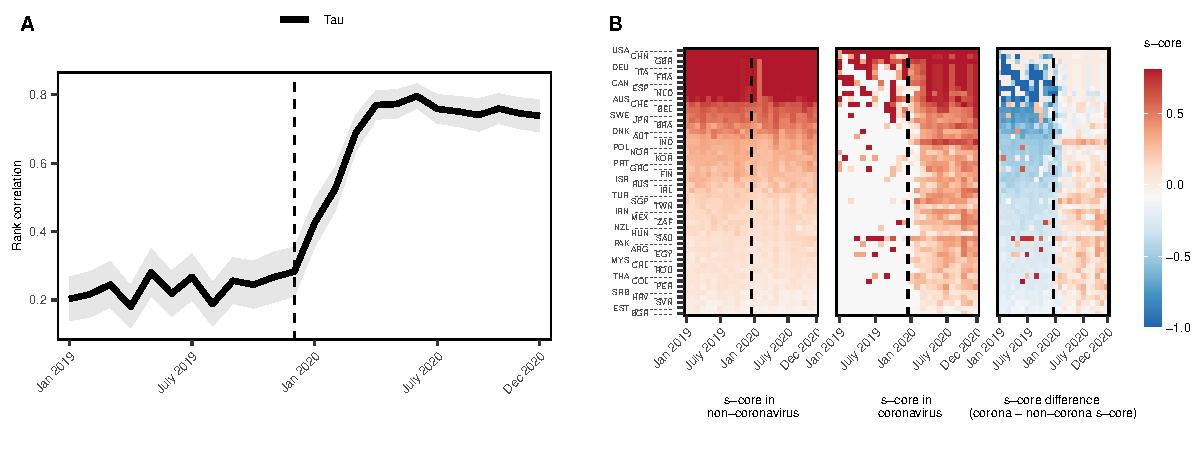
\includegraphics[width=\textwidth]{1_chapter1/figures/Fig3.pdf} %
\caption{{\bf Countries take on the same role in coronavirus research as in the global health sciences.}
{\small (A) Correlation of country rankings by coronavirus and non-coronavirus research by month. (B) Country centrality based on s-core decomposition of the coronavirus and non-coronavirus network by month.}}
\label{figure2} 
\end{figure*}


This trend is consistent with estimation results on the (accumulated) national CRR output (Table~\ref{tab:NationalCRR}), where pre-pandemic health science output ($n_{i,t0}$) becomes the dominant factor from March 2020 on. 


\subsubsection{Network centrality}

% centrality of countries
Similarly, countries' network centrality in the coronavirus research network aligns with their centrality in the overall health science network. 

Fig~\ref{figure2}B provides the monthly s-cores on the non-CRR network (left panel), CRR network (middle panel), and the difference of s-cores in CRR and non-CRR networks (right panel). The figure shows the 60 most central countries in the non-CRR network and applies that same ordering across all three panels. The remaining countries are highly peripheral in either network. 

The left panel of Fig~\ref{figure2}B shows that the global network hierarchy is very stable. The core is formed by developed countries and China. Centrality in the coronavirus network is more dynamic (middle panel). Pre-COVID-19, most countries are not involved in CRR collaborations and, hence, are found in the extreme periphery (white). The core of the CRR network includes only a few of the leading countries in health sciences. On the other hand, Saudi Arabia is part of the core in the CRR network, but peripheral in the overall health science network. The presence of Saudi Arabia in the pre-pandemic CRR network may be explained by previous regional MERS-CoV outbreaks. (Variations in core membership over time may be explained by lower research activity overall which leads to more erratic signals.) After the shock, the structure of the CRR network shifts rapidly towards the hierarchy in health science at large. This is easily seen in the right panel of Fig~\ref{figure2}B that shows the difference between the s-core centrality in the CRR and non-CRR network. Prior to the shock, s-core differences range from -1 in dark blue (for countries at the extreme periphery in the coronavirus network and in the core in the other network), over 0 in white (same s-core in both networks), up to 1 in red (for countries in the CRR network core and peripheral in the non-CRR network). After the shock, the global core rapidly takes its role in CRR, and so does the global periphery (all countries appear in light colors with an s-core difference of around zero from April 2020). 

Closer inspection further reveals that the normalized s-core of more peripheral countries tends to be somewhat higher in the CRR network as in the non-CRR network (Panel `s-core difference' turns rather red than blue in 2020). This means that the distance to the highest core in the network is somewhat reduced. Thus, while the \textit{ranking} by network centrality of countries in the CRR network is maintained as in the non-CRR network, hierarchy has become less steep (at least among the top 60 countries). 


\subsubsection{Network structure}

Fig.~\ref{fig:NetwConvergence} shows how CRR network structure compares to non-CRR network structure over the course of the pandemic. 

Fig.~\ref{fig:NetwConvergence}A provides the correlation coefficient of the (accumulated) CRR and 2019 non-CRR adjacency matrix (in logs) over the observation period. During the pre-pandemic period (2019) the two adjacency matrices are increasingly but only weakly correlated with a coefficient of around 0.25. After the shock in January 2020, within three months (April 2020), the correlation coefficient jumps to 0.75, and increases further to around 0.9 until the end of the analysis period, December 2020. All correlations (pre- and post-pandemic) are highly significant based on a QAP test. Thus, with the COVID-19 pandemic the CRR network structure rapidly approached the prior non-CRR network structure. 

However, the correlation coefficient is not approaching one either, which implies that some structural difference remains between the two networks. So, what's the difference? 

This can be seen in the middle panel (Fig.~\ref{fig:NetwConvergence}B), which provides statistics on network hierarchy ($z_\lambda$) and network modularity ($z_Q$) of the (accumulated) CRR network relative to the prior non-CRR network.

First consider the hierarchy measure $z_\lambda$, the line in red. We start with a $z_\lambda$-value of 1.3 in January 2019 and increase as more CRR collaborations are accumulated up to 7.7 by December 2019. Thus, before the shock the CRR network is more hierarchical than the non-CRR network. This is because only very few countries actually do have some CRR activity making worldwide CRR collaboration highly unequal. In other words, in the land of the blind, the one-eyed man is king. Immediately after the shock, in January 2020 hierarchy increases to $z_\lambda=11.7$. That level of hierarchy is mostly kept in February 2020 but then decreases constantly to attain a value of $z_\lambda=-22.6$ in December 2020, indicating that by the end of 2020 the CRR network is much less hierarchical than the non-CRR network. 

The development of network modularity ($z_Q$) is different. During the pre-pandemic period, 2019, modularity in the CRR network is comparable to modularity in the non-CRR network with a $z_Q$ around zero. This means that pre-pandemic international collaborations on CRR tend to follow the same community structure as pre-pandemic international collaborations on non-CRR.\footnote{Recall that by construction the modularity statistic takes only into account countries that have (any) CRR collaboration.} The first reaction of the community statistic is observed in February 2020 where it jumps on a high level of 6.3 and immediately drops thereafter. Then, from March to December 2020, network modularity increases constantly.

For interpretation we considered $z_Q$ for each community individually (numbers not reported here). The bump of $z_Q$ in February 2020 originates in particular from within cluster interaction in community 1 (in particular USA, China) and to some extent also in community 6 (South America) and community 7 (Middle East and Africa). In contrast, the subsequent more continuous rise of $z_Q$ is driven only by regional communities, i.e. all communities except community 1. In particular community 2 (Central Europe), community 3 (Norther Europe), 6 (South America) and 7 (Middle East and Africa) contribute to this trend.

The panels in Fig.~\ref{fig:NetwConvergence}C show the adjacency matrices of the accumulated CRR network for the three time periods, i.e. the network before the shock in Dec. 2019, immediately after the shock in Feb. 2020, and at the end of the observation period in Dec. 2020. The upper row of panels focusses on the communities. The community panels display the edge weight between two countries above expectations based on their network strength ($w - E(w)$), as used in the community detection algorithm. Countries are ordered by community membership and network centrality, such that squares along the diagonal correspond to communities (the square in the upper left corner corresponds to community 1, the square in the lower right corner to community 7). As the network accumulates, we see that communities become more densely connected. The high $z_Q$ value indicates that the CRR network complies with the modularity structure even more than the (2019) non-CRR network from which these communities have been obtained. 

The lower row of panels gives an impression on the nested hierarchy in the network. Hierarchy plots display the edge weight ($w$) between countries and orders countries from top to down and left to right by their eigenvalue centrality. Nested hierarchy in February 2020 is displayed in the middle panel of the lower row. Given this plot, it is apparent that hierarchy is relatively high mostly because there are very few actors on which IRC activity concentrates. The network of Dec. 2020 is apparently also highly nested, which is a special form of a hierarchical network. However, the low $z_\lambda$ value indicates that the CRR network is in fact less hierarchical (or nested) than the (2019) non-CRR network. 

In sum, by the end of the observation period, the accumulated CRR network has become very similar to the non-CRR network, but less hierarchical and more modular (only) along regional communities. 

%that the CRR network re-establishes modularity to the same extent as the non-CRR network, but remains less hierarchical. Because of a drop in the sample, this observation should be taken with care however.   


%This increase can be traced back to strong IRC activity of US and China (with each other but also with other countries in their cluster). From March to December 2020 network modularity increases constantly. The growth is driven by increased IRC in particular within the South American, Central Europe, and Africa/Middle East clusters. IRC in the cluster including US and China is relatively low.

%During 2019, $z_Q$ decreases only slightly. With the advent of the pandemic in February 2020,  $z_Q$ increases initially from xy to xy, but then undergoes a sharp drop in March 2020 down to xy. It decreases further to its lowest value of xy in July xy, from where on it slightly recovers. Adjacency matrices in Fig.~\ref{figure3}E-G are ordered along the identified communities. Communities correspond to the rectangles on the diagonal. The more collaborations take place outside the diagonals, the more the networks structure deviates from an `ideal' community structure. Even before the shock, Fig.~\ref{figure3}E, the network exhibits clearly no `ideal' community structure as some collaborations are outside the diagonal. In March 2020, Fig.~\ref{figure3}F, the fraction of collaborations outside communities (mostly between core and periphery) increases. Even with the inclusion of more countries into the network in December 2020, communities do not appear to fit particularly well Fig.~\ref{figure3}F. 

%The link formation regression (Table~\ref{tab:jointCRR} estimates strong effects of non-CRR capacity on (accumulated) joint CRR papers ($n_{ij,t0}$, $n_{i,t0}$, $n_{i,t0} + n_{j,t0}$). The overshooting in the hierarchy and the sharp drop in modularity in March 2020 coincides with particularly high estimated coefficients for non-CRR capacity involving not necessarily partners in the past (i.e. $n_{i,t0}$, $n_{i,t0} + n_{j,t0}$). Also, intercepts in February and March 2020 are estimated to be high, suggesting rather exclusive collaboration activities. Later on, mostly from June 2020, several coefficients that are not ultimately connected to prior health science output tend to increase, such as a positive effect of COVID-19 related deaths, closed borders, gdp per capita, and hdi. In combination, these factors reduce network hierarchy without necessarily having strong positive effects on network modularity.

%In the first months after the shock, from January to March 2020, the CRR network becomes much more hierarchical than the non-CRR network ($z_\lambda$ increases up to exp 6). In April 2020 excess hierarchy falls again, comes close to zero in October 2020 (i.e. the hierarchy of the non-CRR network), and further decreases below the non-CRR benchmark in December 2020. Adjacency matrices in Fig.~\ref{figure3}A-C are ordered by eigenvector centrality to visualize the network hierarchy in December 2019 (the state before the pandemic), in March 2020 (highest hierarchy), and December 2020 (end of the analysis period). Comparing Fig.~\ref{figure3}B and Fig.~\ref{figure3}C, one notes that more countries entered the network which naturally reduces hierarchy. 



\begin{figure*}[!h]
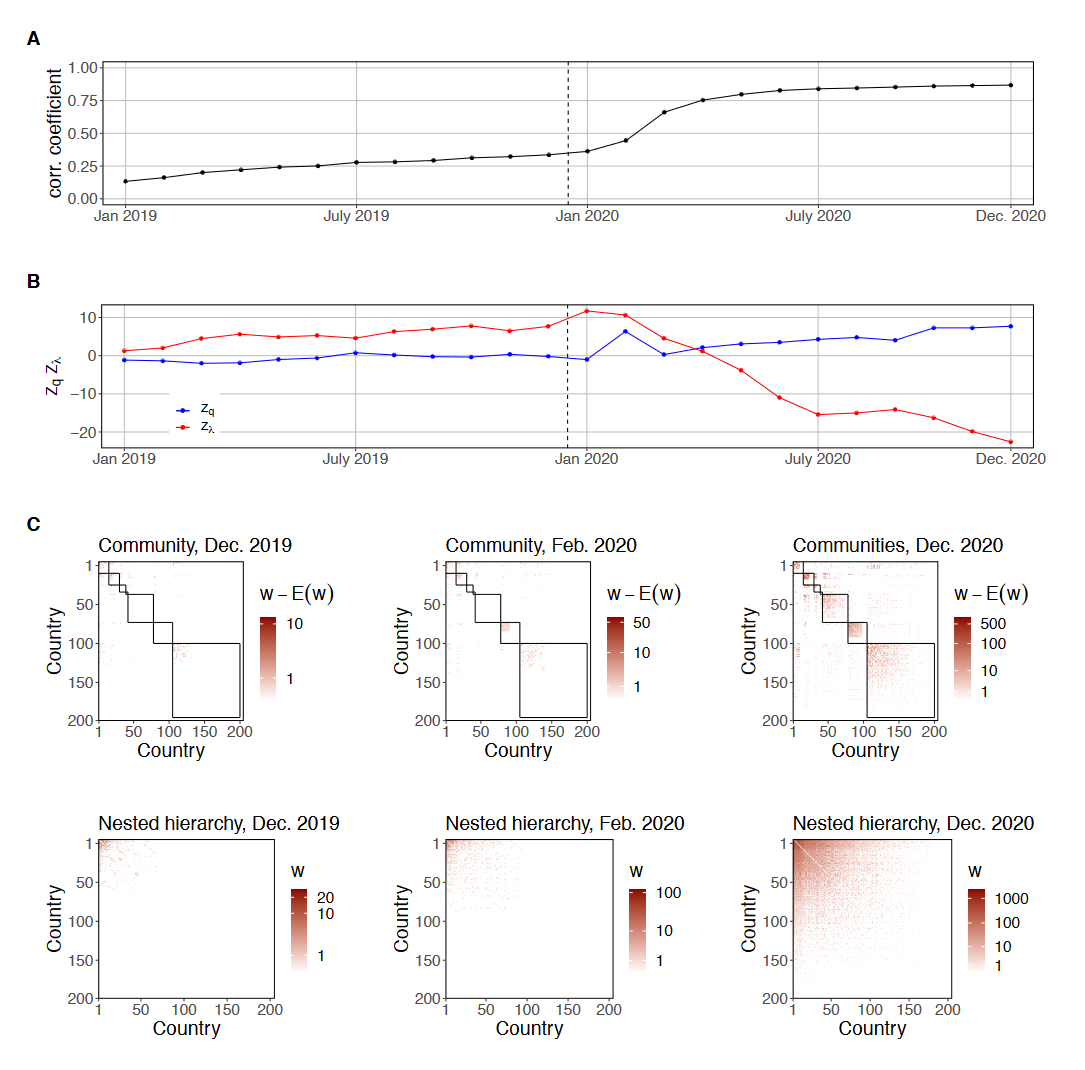
\includegraphics[width=\textwidth]{1_chapter1/figures/Fig4.png} %
\caption{{\bf Convergence of CRR network to non-CRR network.}
{\small In all plots, CRR network is accumulated from Jan. 2019 up to a given month, and the non-CRR network, accumulated from Jan. 2019 to Dec. 2019, serves as the reference network. (A) Pearson's correlation coefficient of (log of) CRR adjacency matrix and non-CRR adjacency matrix. All correlations highly significant according to QAP. (B) Development of $z_q$ (z-value of modularity statistic Q of CRR network with null from non-CRR) and $z_\lambda$ (z-value of largest eigenvalue of CRR network with null from non-CRR network). (C) CRR adjacency matrices arranged by (fixed) communities (upper panels) and nested hierarchy (lower panels). Values in community plots correspond to joint papers in excess of expectations. Values in nested hierarchy plots correspond to the number of joint papers observed. Values mapped to color in log-scale.}}
\label{fig:NetwConvergence} 
\end{figure*}




\section{Discussion and Conclusion}

Based on the population of Medline indexed journal articles, we investigated the global scientific response to the COVID-19 pandemic. Taking an (inter-)national perspective, our analyzes focused on three interrelated aspects: national scientific output, international research collaboration, and network formation. The aim has been to describe the dynamics of CRR during the pandemic and to put them into context. The following first summarizes our main results. Then we turn to the limitations of our study in order to provide policy implications and directions for future research. 

% Main findings:
Our main results may be summarized in three points: % 1. national CRR and international collaboration show the same pattern, they are driven by the same factors and show same dynamics. The strong alignment suggests that one should not see the two as separate activities but rather two dimensions of the same activity. 
First, our three analyses on three different levels yield highly consistent results. Regressions of national CRR output (Analysis 1), and regressions of international collaboration on CRR (Analysis 2), show that national and inter-national scientific activity are closely coupled. Both follow similar dynamics and are driven by essentially the same factors. Analysis 3 on the international CRR network describes the order of global CRR that emerges as a consequence. The close coupling of national and international positioning in CRR is in strong agreement with the broader literature on (inter-)national science systems \citep[see e.g.][in combination]{adams2013fourth,davidson1977distribution,luukkonen1992understanding,pan2012world,gui2018international}.

% 2. The regression analyses show a shift from CRR to non-CRR capacity as the dominating driver. Other factors are less important
Second, regression analyses 1 and 2 show that CRR specific science capacity accumulated before the pandemic has been influential for national CRR output and international CRR collaboration in particular during the first three months of the pandemic. Broader health science capacity has become the dominant factor for (inter-)national CRR at least two months after the beginning of the pandemic. Pandemic related contextual factors, COVID-19 related deaths, lockdowns, and border closure, have been estimated to be systematically and positively correlated with (inter-)national CRR output mostly in the second half of 2020. These effects remain small however compared to broader health science capacity. Similarly, socio-economic conditions, i.e. population size, GDP per capita, and human development (HDI), do take some but limited explanatory power over the course of the pandemic. Regression analysis 2 further shows a strong effect of being located in the same region on international CRR collaboration. 

We thus complement prior, more qualitative, studies. \citet{haghani2020covid} and \citet{zhang2020scientific} show that pre-pandemic CRR and non-CRR both provide relevant knowledge for the COVID-19 pandemic. Our regressions show a clear order in time of how coronavirus specific knowledge and more general health science capacity has been leveraged. The role of pandemic related factors has been put forward to explain observations on (inter-)national CRR in several studies \citep{haghani2020covid,fry2020consolidation,zhang2020scientific}. For example the dynamics of the infection process has been related to dynamics in CRR output in particular for China and Italy \citep[e.g.][]{fry2020consolidation}. While pandemic related explanations may well hold for individual countries, we find that such effects are \textit{on average} relatively small. This can be explained with the fact that the global scientific community rapidly felt some urgency. Similarly, the relatively small effect of GDP and HDI suggest that, in the short run, science capacity is largely fixed. Our estimates on the relevance of regional collaboration complies with the general literature on IRC \citep{frenken2009spatial} as well as observations on regional epidemics \citep{haghani2020covid,zhang2020scientific}. %Thus, a systematic `region' effect during the global pandemic COVID-19 seems natural.
 
% 3. Consequently, global CRR during the pandemic converges towards global non-CRR before the pandemic. 
Third, consistent with regression results, Analysis 3 shows that global CRR during the pandemic rapidly converges towards the global order of broader health science capacity. Within three months, country rankings by national CRR output approach rankings by pre-pandemic non-CRR output (Analysis 3.1), countries take the same (centrality) position in the international CRR network as in the pre-pandemic broader health science network (Analysis 3.2), and the CRR network converges to the structure of the pre-pandemic health science network (Analysis 3.3).  % 4. There is a systematic deviation of CRR network from non-CRR network. CRR network is less hierarchic and emphasizes more regional communities. 
However, the alignment is not perfect. Global CRR deviates systematically from the attracting global distribution of broader health science before the pandemic in that the global CRR network is significantly less hierarchic and more regional than global health science (Analysis 3.3).  

These results are all consistent with prior empirical studies on the expansion of the international CRR network \citep{cai2021international,fry2020consolidation,haghani2020covid,zhang2020scientific}. Our study clarifies however that the pre-existing global health science system systematically structures the expansion of global CRR, and add that global CRR systematically deviates in relevant dimensions from the inherited global structure.


One major limitation of this study is the arguably rough division of research papers into two categories; CRR and non-CRR. The following discussion takes this limitation into account to delineate policy implications and to outline potential avenues for future research. 

% 2. No distance measured from prior research activity to CRR research, and hence we can say nothing about the degree of flexibility in the science system. Therefore we do not know whether flexibility arouse from basic science (generic knowledge) or from occupying research topics that are somewhat close (to some dimension) of the pandemic. 
The COVID-19 shock opened a scientific race. In order to start off, most scientists had to re-orient or adapt ongoing research. Our observation that countries with prior experience in CRR occupied pole positions but countries of the global health science core rapidly took the lead, suggests that a broad science base provides the ability to re-orient research effectively. This is an argument for a more autonomous development of the science system, because it deliberates policy and society from the burden (and impossibility) to specify a detailed scientific agenda to meet future challenges. 

However, having no notion of distance between non-CRR and CRR, we can say nothing about the degree of flexibility in research orientation, nor what exactly underlies such flexibility. In particular we would like to know to what extent CRR research during the pandemic benefited from very generic scientific capacity (obtained through basic science), from closely related scientific capacity (broad array of applied sciences somehow related to CRR), or their interaction. This would give some indication for science policy on how to balance basic science against applied research to guard against future challenges. 

Immediately after the shock the need for international collaboration has been emphasized by all stakeholders. Our results show that national CRR output and international CRR collaboration have been so closely aligned that they should be considered as two dimensions of the same activity. Furthermore, we found that the international collaboration network on CRR largely followed the prior international health science network. The implication is that any (national) strategy to develop science capacity must take a (global) systems perspective --- the embedding of the national science system in the international collaboration network is part of the (slowly accumulating and path dependent) national science base. 

It is hard to spell out that insight without raising two follow-up questions: What would be an `appropriate' network structure (and for whom)? How could such an `appropriate' network structure be obtained? Our observation that the international CRR network systematically deviates from the broader health science network may help to scratch on these issues --- but with major limitations. 

According to our analysis, the international CRR network exhibits a less steep hierarchy and stronger regionalization than the international broader health science network. Yet, what exactly that signifies remains unclear. Recall that we do not differentiate papers by quality, we only measure quantities. COVID-19 has been a hot science topic in 2020, and it may be that many papers have been hastingly crafted but add little knowledge. A higher propensity of low quality papers in countries with lower scientific capacity could contribute to our finding of a less steep global hierarchy as measured on output quantity, while global hierarchy in terms of research excellence may be in fact maintained. Similarly, increased regionalization, as we observe it, is consistent with more independent science in the different world regions and hence more independent accumulation of science capacity on a regional level. But it is also consistent with maintained but unresolved resource (inter-)dependence and increasing vertical stratification (by scientific excellence) as well as horizontal stratification (by research topics). Thus, the paper at hand clearly describes structural changes, but leaves the question of individual network gains and global network efficiency for future research. 

Finally, the underlying cause of structural changes in global CRR remains unclear. On the one hand, stronger regionalization may be largely due to the pandemic context. Our regressions include relevant parameters such as national pandemic policy measures and virus spreading dynamics, but these are certainly no perfect controls. Given those controls bite, our results are consistent with the idea that we observe the accentuation of a long-term trend towards regionalization; a trend already observed by \citet{fitzgerald2021academia} for the sciences in general. In case the pandemic context is the underlying cause, the organization of global science during the pandemic may be as transitory as the pandemic itself. If the organization of global CRR during the pandemic accentuates a general global trend, it may not only cast the shadow of a future multi-polar world but even accelerate that trend. 




%\begin{acknowledgements}
%If you'd like to thank anyone, place your comments here
%and remove the percent signs.
%\end{acknowledgements}


% Authors must disclose all relationships or interests that 
% could have direct or potential influence or impart bias on 
% the work: 
%
% \section*{Conflict of interest}
%
% The authors declare that they have no conflict of interest.


% BibTeX users please use one of
%\bibliographystyle{spbasic}      % basic style, author-year citations
%\bibliographystyle{spmpsci}      % mathematics and physical sciences
%\bibliographystyle{spphys}       % APS-like style for physics
%\bibliography{}   % name your BibTeX data base



\clearpage
\newpage


\section{Appendix}

\subsection{Sample}
\label{sec:AppendixSample}

\subsection{Timelags from research over acceptance to entry into the PubMed dataset}
\label{subsec:Timelags}

\begin{figure*}[!h]
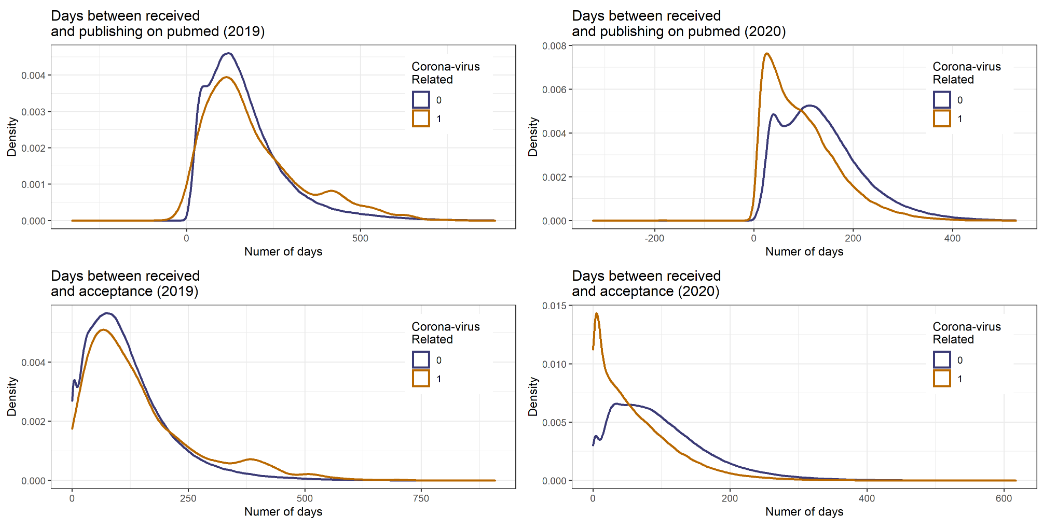
\includegraphics[width=\textwidth]{1_chapter1/figures/Fig5.png} %
\caption{{\bf Timelags from submission date (data received) to (clockwise, starting with the upper left panel): i) publishing on PubMed in 2019, ii) publishing on PubMed in 2020, iii) journal acceptance in 2020, iv) journal acceptance in 2019.} \textit{Our sample is from PubMed. Therefore, the analysis period is based on the timelag distribution of the upper right panel.}}
\label{fig:Timelags} 
\end{figure*}


\begin{landscape}

\begin{table}[t!]\footnotesize
\centering  
\caption{Descriptive statistics on scientific production (at submission date)}
\begin{threeparttable}
\label{tab:DescriptivesSciProd} 
\begin{tabular}{@{\extracolsep{-7pt}} lcccccc} 
\hline
& \multicolumn{2}{c}{\textit{Coronavirus related}} 
& \multicolumn{2}{c}{\textit{Others Documents}}
& \multicolumn{2}{c}{\textit{All Documents}} \\ 
\cline{2-7} 
\\[-1.8ex] & \multicolumn{1}{c}{2019}
&\multicolumn{1}{c}{2020}
&\multicolumn{1}{c}{2019}
& \multicolumn{1}{c}{2020}
&\multicolumn{1}{c}{2019}
&\multicolumn{1}{c}{2020} \\ 
  \hline
  \\[5pt]
  Nb of authors & 6/7.36 (4.86) & 5/6.86 (7.05) & 6/6.66 (17.51) & 6/6.65 (14.67) & 6/6.66 (17.5) & 6/6.66 (14.2) \\ 
  \\[5pt]
  Solo authors  & 2.83 & 6.72 & 3.38 & 3.22 & 3.38 & 3.5\\
    \\[5pt]
  International collab.  & 25.44 & 23.06 & 23.57 & 23.63 & 23.57 & 23.58) \\ 

\\[5pt]
  Nb of country & 1/1.36 (0.92) & 1/1.35 (1.29) & 1/1.31 (1.05) & 1/1.32 (1.01) & 1/1.31 (1.05) & 1/1.33 (1.03) \\ 
\\[5pt]
 Days received-accept & 110.04/143.31 (119.52) & 45/60.87 (58.53) & 99.96/118.97 (93.82) & 84.96/97.96 (73.24) & 99.96/119 (93.85) & 81.96/94.88 (72.86) \\ 
  \\[5pt]
 Share aff. captured & 1/0.95 (0.2) & 1/0.92 (0.26) & 1/0.93 (0.24) & 1/0.95 (0.21) & 1/0.93 (0.24) & 1/0.94 (0.22) \\ 

  \hline
   \# Document & 743(0.1\%) & 74250(8.2\%) & 775738(99.9\%) & 830914(91.8\%) & 776481 & 905164\\
  \hline
  \end{tabular}
  \begin{tablenotes}
  \footnotesize
  \item {\it Notes:} Binary indicators in [\%], for continuous measures [median/mean (s.d.)].
  \end{tablenotes}
 \end{threeparttable}
\end{table}

\end{landscape}



\subsection{Regression analysis: Marginal effects}
\label{sec:MargEffects}


Marginal effects of the zero-inflated negative binomial regression of (accumulated) joint CRR papers are obtained from the estimated coefficient in Table~\ref{tab:jointCRR}. To keep it simple, we calculate numerically to what extent a `small' increase in the value of one variable affects on average the expected outcome.\footnote{Note that we cannot calculate significance values of the marginal effects by using the `Delta' method, because standard deviations based on asymptotics are not reliable (see Methods).} For all variables, except for the `same region' dummy, a small increase is considered to be a one percent increase of the observed value (before taking logs). Observations with value zero are shifted to one. The marginal effect for one observation is then the ratio of the prediction based on the increased value over the prediction based on the originally observed value.  The dummy variable `same region' is the exception in that we compare the expected outcome based on a value of zero (not in same region) with the expected outcome based on a value of one (same region) for each observation. The average marginal effect is the average over all individual marginal effects. 

Table~\ref{tab:margEff} provides the average marginal effects obtained for each regression. As a reading example, we discuss the marginal effects of factors with `significant' coefficients in the February 2020 regression in Table~\ref{tab:jointCRR}: In terms of average marginal effects, a one percent increase of ($n_{i,t0} + n_{j,t0}$) translates into a 1.1 percent increase of expected joint CRR papers. Average marginal effect of `same region' appears to be large: On average, being located in the same region, rather than not, increases the expected number of joint CRR papers by about four times (i.e. 384 percent).\footnote{The high marginal effect of the `same region' dummy variable compared to the marginal effects of other variables with comparable coefficient estimates is due to the binary nature of the dummy. Marginal effects of the dummy are based on a comparison of zero value to a value of one. For all other variables, average marginal effects are calculated on a one percent increase of the underlying variable, before taking logs for estimation. This corresponds to adding one percent (0.01) after taking logs. Thus, we consider a step size for the dummy variable `same region' that is 100 times larger as for all other variables.}

Looking at the count model of the intensity of dyadic CRR, we estimate a significant coefficient of one for joint non-CRR in the prior year 2019. A one percent increase of that variable translates into an expected increase of the outcome by around 36 percent. On the other hand, a one percent increase of (sole) non-CRR papers reduces the expected outcome by half a percent. Countries with specific CRR capacity attract collaborators ($c_{i,t0}$) in that a one percent increase is expected to increase the outcome by seven percent. A one percent increase of country size (pop) and economic wealth (gdp per capita) shift average expected outcomes by 0.25 percent and 0.65 percent respectively. One percent increases of ($hdi_i + hdi_j$) and ($|hdi_i - hdi_j|$) reduce the outcome by 1.9 and 0.5 percent respectively. 

Considering the table as a whole, we see that being located in the same region and having many prior non-CRR ties are associated with the largest marginal effects. 

\begin{landscape}

% latex table generated in R 3.6.3 by xtable 1.8-4 package
% Mon Aug  2 17:30:54 2021
\begin{table}[ht]
\caption{Marginal effects of zero-inflated negative binomial regression of (accumulated) joint CRR papers (in percent).}
\label{tab:margEff}
\centering
\begin{threeparttable}
\begin{tabular}{rrrrrrrrrrrr}
  \hline
    & {\bf Feb. `20} & {\bf Mar. `20} & {\bf Apr. `20} &  {\bf May `20}  &  {\bf June `20} &  {\bf July `20} &  {\bf Aug. `20} &  {\bf Sept. `20} &  {\bf Oct. `20} &  {\bf Nov. `20} &  {\bf Dec. `20}   \\ 
  \hline
    $n_{ij,t0}$ & 39.02 & 21.66 & 27.53 & 28.96 & 25.45 & 23.77 & 23.55 & 23.80 & 24.04 & 24.54 & 25.07 \\ 
     $c_{ij,t0}$ & 12.53 & 3.03 & 0.33 & 0.37 & 3.68 & 4.06 & 3.92 & 2.36 & 1.72 & 1.91 & 1.74 \\ 
  $n_{i,t0}$  & -0.53 & 0.26 & 0.09 & 0.04 & 0.15 & 0.17 & 0.17 & 0.17 & 0.15 & 0.15 & 0.14 \\ 
     $c_{i,t0}$ & 7.01 & 0.39 & 0.86 & 1.05 & -0.06 & 0.11 & 0.16 & 0.48 & 0.67 & 0.33 & 0.36 \\ 
  $death_i + death_j$ & -43.25 & 0.13 & 0.12 & 0.08 & 0.08 & 0.10 & 0.12 & 0.14 & 0.18 & 0.15 & 0.14 \\ 
  $|death_i - death_j|$ & 94.60 & -0.28 & -0.13 & -0.05 & -0.04 & -0.06 & -0.06 & -0.08 & -0.10 & -0.08 & -0.08 \\ 
  $locked_{i,t'}$  & -3.95 & 1.75 & 1.27 & 1.00 & 0.74 & 1.14 & 0.84 & 0.77 & 0.80 & 0.63 & 0.65 \\
  $closed_{i,t'}$ &  & 0.46 & 0.10 & 0.03 & 0.05 & 0.08 & 0.11 & 0.11 & 0.11 & 0.10 & 0.10 \\ 
  $pop_{i,t0}$ & 0.23 & -0.01 & 0.04 & 0.03 & -0.01 & 0.01 & 0.02 & 0.00 & 0.01 & 0.02 & 0.02 \\
  $gdp_i + gdp_j$ & 0.67 & 0.41 & 0.16 & 0.07 & 0.22 & 0.23 & 0.31 & 0.33 & 0.30 & 0.34 & 0.34 \\ 
  $|gdp_i - gdp_j|$ & 0.06 & 0.03 & 0.05 & 0.05 & 0.05 & 0.04 & 0.04 & 0.04 & 0.04 & 0.03 & 0.04 \\
  $hdi_i + hdi_j$ & -2.03 & -2.09 & -0.92 & -0.88 & -1.64 & -1.55 & -1.73 & -1.81 & -1.64 & -1.75 & -1.75 \\ 
  $|hdi_i - hdi_j|$  & -0.49 & -0.37 & -0.42 & -0.36 & -0.42 & -0.41 & -0.43 & -0.43 & -0.41 & -0.42 & -0.42 \\ 
   $n_{i,t0} + n_{j,t0}$   & 1.08 & 3.27 & 1.21 & 0.95 & 0.84 & 0.99 & 1.00 & 0.97 & 1.18 & 1.04 & 0.99 \\ 
  $|n_{i,t0} - n_{j,t0}|$ & -0.38 & -2.62 & -0.66 & -0.43 & -0.41 & -0.55 & -0.56 & -0.52 & -0.69 & -0.55 & -0.50 \\ 
  distance & 0.02 & 0.30 & -0.16 & -0.22 & -0.14 & -0.18 & -0.22 & -0.20 & -0.20 & -0.20 & -0.17 \\ 
  same region & 339.05 & 464.83 & 615.06 & 422.27 & 235.25 & 225.90 & 206.43 & 237.96 & 245.15 & 231.95 & 234.30 \\ 
   \hline
\end{tabular}
  \begin{tablenotes}
  \footnotesize
  \item {\it Notes: Average marginal effects have been obtained by comparing for each variable predictions based on observations with predictions on observed increased by one percent. In case observed value is zero, we compare it with having one. Marginal effects of the dummy `same region' are obtained by comparing zero with one outcomes.}
  \end{tablenotes}
 \end{threeparttable}
\end{table}

\end{landscape}


\subsection{Community detection in the 2019 non-CRR network}
\label{Appendix:Communities}

The procedure is the same as in \citet{FitzgeraldEtAl2021}, but relevant details are repeated here for readers' convenience.

We identify communities with the spin glass community detection algorithm of \cite{ReichardtBornholdt2006}. The objective criterion to be maximized is 

\begin{equation*}
	Q = \frac{1}{m} \left( \sum_{ij} c_{ij} - \gamma \frac{k_i k_j}{m} \right) d(\sigma_i,\sigma_j) \text{,} 
\end{equation*}

where $m$ is the sum over all edges, $c_{ij}$ is the number of joint papers between country $i$ and $j$, $k_i$ ($k_j$) is the strength of country $i$ ($j$) (i.e. the sum over all weighted edges of the country), $\sigma_i$ ($\sigma_j$) indicates the community of $i$ ($j$) in a given network partition, with the function $d()$ evaluating to one if both countries belong to the same community (i.e. $\sigma_i = \sigma_j$) and zero else. Finally, the tuning parameter $\gamma$ trades-off the two objectives of having high edge weights within clusters against having few edge weights between clusters. A smaller (higher) $\gamma$ tends to yield less (more) clusters. 

The optimization is done through simulated annealing (as implemented in the R-package `igraph'). Simulated annealing is a stochastic optimization algorithm and hence may provide different partitions for the same data and parameter settings. In order to find robust communities,  we run many (i.e. 100) times the optimization algorithm over a grid of $\gamma$, starting from 0.8 to 1.6. The resulting community partitions for a given $\gamma$ are then compared, each partition against all others. Similarity of two partitions is measured by the `Variation of Information' (VI). The following definition is paraphrased from \citep[][Appendix 4]{FitzgeraldEtAl2021}:

``\textit{Consider two partitions $X$ and $Y$ of a set $A$ into disjoint subsets, $X={X_1,X_2,\ldots,X_k}$ and $Y={Y_1,Y_2,\ldots,Y_l}$, VI is defined as follows. Let $n=\sum_i |X_i|=\sum_j |Y_j|=|A|$, $p_i=|X_i| / n$, $q_j = |Y_j| / n$, $r_{ij}=| X_i \cap Y_j| / n$. Then the normalised variation of information between the two partitions is:}

\begin{equation*}
	VI(X,Y) = - 1 \log N \sum_{i,j} r_{ij} \left[ \log(r_{ij}/p_i) + \log(r_{ij}/q_j) \right] \text{.''}
\end{equation*}
 
Table \ref{tab:VI} provides the VIs for 100 optimizations for each $\gamma$ on the grid. The most robust partitioning is obtained for $\gamma=0.8$. The resolution of that partitioning however is very low, dividing the world into one cluster of less developed economies (consisting of countries in Africa, Middle East, South Asia, and India, Mongolia, and Kazakhstan) and another cluster including all other countries. The partitioning with $\gamma=1.2$ is slightly less robust but at much higher resolution. Figure~\ref{fig:CommWorldmap} shows the partitioning with lowest average VI under $\gamma=1.2$. We choose that partition as our benchmark. Interestingly, the partitioning that we obtain on the 2019 non-CRR network is not identical but very similar to the partitioning obtained by \citet[][Fig.5b]{FitzgeraldEtAl2021} based on all Scopus publications in 2015. 



\begin{table}[ht]
\caption{Variation of Information for varying $\gamma$ over 100 optimizations.}
\label{tab:VI}
\centering
\begin{tabular}{cccccccccc}
  \hline
$\gamma$ & 0.8 & 0.9 & 1.0 & 1.1 & 1.2 & 1.3 & 1.4 & 1.5 & 1.6 \\ 
    \hline
VI & 0.099 & 0.302 & 0.465 & 0.161 & 0.102 & 0.349 & 0.255 & 0.158 & 0.232 \\ 
\hline
\end{tabular}
\end{table}


The partitioning displayed in Figure~\ref{fig:CommWorldmap} consists out of the following communities (ordered by average degree of their members):

\begin{enumerate}
	\item[Cluster 1:]	Australia, Canada, China, French Polynesia, Gibraltar, Grenada, Japan, Macao SAR China, New Zealand, Singapore, Solomon Islands, South Korea, Taiwan, United Kingdom, United States 
	\item[Cluster 2:] Austria, Belgium, Curacao, France, Germany, Italy, Liechtenstein, Luxembourg, Martinique, Monaco, Netherlands, Réunion, Spain, Switzerland, Vatican City 
	\item[Cluster 3:] Denmark, Faroe Islands, Finland, Greenland, Guinea-Bissau, Iceland, Isle of Man, Norway, Sweden 
	\item[Cluster 4:] Israel, Jersey, Montserrat 
	\item[Cluster 5:] Albania, Angola, Armenia, Azerbaijan, Belarus, Bosnia \& Herzegovina, Bulgaria, Croatia, Cyprus, Czechia, Estonia, Georgia, Greece, Hungary, Ireland, Kazakhstan, Latvia, Lithuania, Malta, Moldova, Montenegro, North Macedonia, Poland, Portugal, Romania, Russia, San Marino, Serbia, Sint Maarten, Slovakia, Slovenia, Tajikistan, Turkey, Turkmenistan, Ukraine, Uzbekistan 
	\item[Cluster 6:] Andorra, Antigua \& Barbuda, Argentina, Belize, Bolivia, Brazil, Chile, Colombia, Costa Rica, Cuba, Dominica, Dominican Republic, Ecuador, El Salvador, French Guiana, Guatemala, Guyana, Honduras, Mexico, Nicaragua, Panama, Paraguay, Peru, St. Kitts \& Nevis, Suriname, Uruguay, Venezuela 
	\item[Cluster 7:] Afghanistan, Algeria, Aruba, Bahamas, Bahrain, Bangladesh, Barbados, Benin, Bermuda, Bhutan, Botswana, Brunei, Burkina Faso, Burundi, Cape Verde, Cambodia, Cameroon, Cayman Islands, Central African Republic, Chad, Congo - Kinshasa, Egypt, Eritrea, Ethiopia, Fiji, Gabon, Gambia, Ghana, Guadeloupe, Guinea, Haiti, India, Indonesia, Iran, Iraq, Côte d?Ivoire, Jamaica, Jordan, Kenya, Kuwait, Kyrgyzstan, Laos, Lebanon, Lesotho, Liberia, Libya, Madagascar, Malawi, Malaysia, Maldives, Mali, Mauritania, Mauritius, Mongolia, Morocco, Mozambique, Myanmar (Burma), Namibia, Nepal, New Caledonia, Niger, Nigeria, Oman, Pakistan, Palau, Palestinian Territories, Philippines, Qatar, Congo - Brazzaville, Rwanda, St. Lucia, St. Vincent \& Grenadines, Samoa, Saudi Arabia, Senegal, Seychelles, Sierra Leone, Somalia, South Africa, Sri Lanka, Sudan, Syria, Tanzania, Thailand, Togo, Tonga, Trinidad \& Tobago, Tunisia, Turks \& Caicos Islands, Uganda, United Arab Emirates, Vietnam, Yemen, Zambia, Zimbabwe 
	\item[No cluster:] Djibouti, \"Aland Islands, British Virgin Islands, Sao Tome and Principe, Tuvalu
\end{enumerate}


\subsection{Extended analysis up to April 2021}
\label{sec:ExtAnalysis}


% latex table generated in R 3.6.3 by xtable 1.8-4 package
% Fri Jul 30 23:19:16 2021

\begin{table}[h!]
	\begin{threeparttable}
\centering
\caption{National output regression (Jan.-Apr. 2021).}
\label{tab:NationalCRRExtended}
\begin{small}
\begin{tabular}{lcccc}
\hline\noalign{\smallskip}
  & {\bf Jan.} & {\bf Feb.} & {\bf Mar.} & {\bf Apr.} \\
  \hline
  & {\bf`21}   & {\bf`21}     & {\bf`21}.    & {\bf`21} \\
  \hline
   $n_{t0}$ & 0.946 ***  & 0.946 ***  & 0.948 ***  & 0.952 ***  \\ 
   & (0.05) & (0.05) & (0.048) & (0.049) \\ 
   $c_{t0}$ & 0.016   & 0.015   & 0.01   & 0.007   \\ 
   & (0.036) & (0.036) & (0.035) & (0.036) \\ 
  $deaths_{t'}$ & 0.052   & 0.049   & 0.043   & 0.035   \\ 
   & (0.029) & (0.029) & (0.028) & (0.029) \\ 
  $locked_{t'}$ & 0.06 **  & 0.064 **  & 0.066 ***  & 0.066 **  \\ 
   & (0.02) & (0.02) & (0.019) & (0.02) \\ 
$border_{t'}$ & -0.013   & -0.015   & -0.016   & -0.015   \\ 
   & (0.021) & (0.021) & (0.02) & (0.02) \\ 
  $pop_{t0}$ & 0.007   & 0.004   & 0.011   & 0.015   \\ 
   & (0.04) & (0.04) & (0.039) & (0.04) \\ 
  $gdp_{t0}$ & 0.114 *  & 0.11 *  & 0.12 *  & 0.123 *  \\ 
   & (0.053) & (0.052) & (0.051) & (0.052) \\ 
  $hdi_{t0}$ & -0.159 **  & -0.151 **  & -0.156 **  & -0.155 **  \\ 
   & (0.058) & (0.057) & (0.056) & (0.057) \\ 
\noalign{\smallskip}\hline\noalign{\smallskip}
$R^2$ & 0.947 & 0.948 & 0.951 & 0.95 \\ 
\noalign{\smallskip}\hline\noalign{\smallskip}

\end{tabular}
  \end{small}
    \begin{tablenotes}
  \footnotesize
  \item {\it Notes:} Recall from Section \ref{subsec:Analysis1} that $c_{t0}$ and $n_{t0}$ proxy initial scientific capacity in CRR and non-CRR respectively. 
    \end{tablenotes}
  \end{threeparttable}
\end{table}


\begin{table}[ht]
\begin{threeparttable}
\centering
\caption{Zero-inflated negative binomial model of (accumulated) joint coronavirus related papers (Jan.-Apr. 2021), est. coefficient (z-value, p-value)}
\label{tab:jointCRR_extended}
\begin{small}
\begin{tabular}{rllll}
\hline\noalign{\smallskip}
  & {\bf Jan. `20}  & {\bf Feb. `20} & {\bf Mar. `20} & {\bf Apr. `20}    \\ 
\noalign{\smallskip}\hline\noalign{\smallskip}
       	\textit{Count-model} & & & &  \\
\noalign{\smallskip}
Intercept & -4.023*** & -3.885*** & -3.99*** & -4.062*** \\ 
   & (-12.164, 0) & (-12.163, 0) & (-12.544, 0) & (-12.772, 0) \\ 
  $n_{ij,t0}$ & 0.75*** & 0.751*** & 0.752*** & 0.744*** \\ 
   & (50.115, 0) & (51.896, 0) & (52.291, 0) & (51.752, 0) \\ 
    $c_{ij,t0}$ & 0.032 & 0.025 & 0.022 & 0.024 \\ 
   & (0.76, 0.248) & (0.622, 0.321) & (0.535, 0.31) & (0.581, 0.343) \\ 
  $n_{i,t0}$ & 0.149*** & 0.135** & 0.139*** & 0.149*** \\ 
   & (9.859, 0) & (9.315, 0.001) & (9.594, 0) & (10.317, 0) \\ 
  $c_{i,t0}$  & 0.006 & 0.01 & 0.006 & 0.006 \\ 
   & (0.492, 0.458) & (0.857, 0.393) & (0.482, 0.47) & (0.467, 0.434) \\ 
   $death_i + death_j$ & 0.112** & 0.106** & 0.101** & 0.101** \\ 
   & (6.177, 0.004) & (6.165, 0.006) & (6.027, 0.009) & (5.867, 0.009) \\ 
   $|death_i - death_j|$ & -0.059* & -0.056* & -0.055* & -0.056* \\ 
   & (-4.181, 0.038) & (-4.214, 0.036) & (-4.327, 0.035) & (-4.247, 0.034) \\ 
  $locked_{i,t'}$ & 0.028* & 0.03** & 0.031** & 0.03** \\ 
   & (6.364, 0.014) & (7.323, 0.005) & (7.779, 0.001) & (7.627, 0.009) \\ 
 $closed_{i,t'}$ & 0.025** & 0.022** & 0.021** & 0.022** \\ 
   & (6.596, 0.005) & (5.95, 0.009) & (5.766, 0.006) & (6.092, 0.007) \\ 
     $pop_{i,t0}$ & 0.023 & 0.027 & 0.031 & 0.029 \\ 
   & (1.953, 0.224) & (2.359, 0.186) & (2.653, 0.133) & (2.484, 0.172) \\ 
  $gdp_i + gdp_j$ & 0.358*** & 0.359*** & 0.385** & 0.396** \\ 
   & (7.735, 0) & (8.007, 0) & (8.609, 0.001) & (8.83, 0.001) \\ 
  $|gdp_i - gdp_j|$ & 0.033 & 0.037 & 0.037 & 0.036 \\ 
   & (2.789, 0.121) & (3.183, 0.069) & (3.194, 0.087) & (3.103, 0.078) \\ 
 $hdi_i + hdi_j$ & -2.363*** & -2.21*** & -2.285*** & -2.348*** \\ 
   & (-12.007, 0) & (-11.588, 0) & (-12.033, 0) & (-12.348, 0) \\ 
 $|hdi_i - hdi_j|$ & -1.835*** & -1.834*** & -1.867*** & -1.848*** \\ 
   & (-11.816, 0) & (-12.17, 0) & (-12.443, 0) & (-12.325, 0) \\ 
  distance & -0.044 & -0.064* & -0.071* & -0.077* \\ 
   & (-2.525, 0.16) & (-3.848, 0.034) & (-4.233, 0.024) & (-4.576, 0.023) \\ 
  same region & 0.165*** & 0.175*** & 0.168*** & 0.163*** \\ 
   & (5.152, 0) & (5.687, 0) & (5.446, 0) & (5.276, 0) \\ 
     $log(\theta)$  & 1.251*** & 1.322*** & 1.295*** & 1.275*** \\ 
 & (28.604, 0) & (30.667, 0) & (30.729, 0) & (30.595, 0) \\ 
   \noalign{\smallskip}\hline\noalign{\smallskip}
      	\textit{Zero-model} & & & &  \\
\noalign{\smallskip}
     Intercept & 7.56*** & 7.091*** & 7.533*** & 7.323*** \\ 
   & (6.181, 0) & (5.87, 0) & (6.235, 0) & (6.045, 0) \\ 
  $n_{i,t0} + n_{j,t0}$ & -2.972** & -2.998*** & -3.031** & -3.064** \\ 
   & (-9.464, 0.002) & (-9.845, 0) & (-10.001, 0.002) & (-9.753, 0.009) \\ 
  $|n_{i,t0} - n_{j,t0}|$ & 1.448** & 1.45** & 1.457** & 1.502** \\ 
   & (5.18, 0.004) & (5.35, 0.002) & (5.412, 0.001) & (5.354, 0.001) \\ 
  distance & 0.471** & 0.547** & 0.518** & 0.532** \\ 
   & (3.894, 0.003) & (4.551, 0.002) & (4.299, 0.002) & (4.375, 0.005) \\ 
  same region & -2.492*** & -2.57*** & -2.704*** & -2.797*** \\ 
   & (-7.476, 0) & (-7.988, 0) & (-8.462, 0) & (-8.274, 0) \\ 
\noalign{\smallskip}\hline\noalign{\smallskip}
  obs. & 12090 & 12090 & 12090 & 12090 \\ 
  loglik & -15655 & -15885 & -16075 & -16199 \\ 
\noalign{\smallskip}\hline\noalign{\smallskip}
\end{tabular}
   \end{small}
       \begin{tablenotes}
  \footnotesize
  \item --- P-values are based on MRQAP (1000 permutations) and one-sided (because null distributions are not symmetric). One, two, and three stars signal significance values below 5\%, 1\%, and 0.1\% respectively. Marginal effects are in Appendix~\ref{sec:MargEffects}, Table~\ref{tab:margEff}.
  \item --- Recall from Section \ref{subsec:Analysis2} that $n$ and $c$ stands for non-CRR and CRR respectively. Indices $i$ indicate a country, and $ij$ a country dyad. Country-level variables are joined to capture the country dyad's sum ($x_i + x_j$) and their absolute difference ($|x_i - x_j|$).  $log(\theta)$ captures over-dispersion in the count model.
    \end{tablenotes}
\end{threeparttable}
\end{table}



\clearpage






\begin{figure*}[!h]
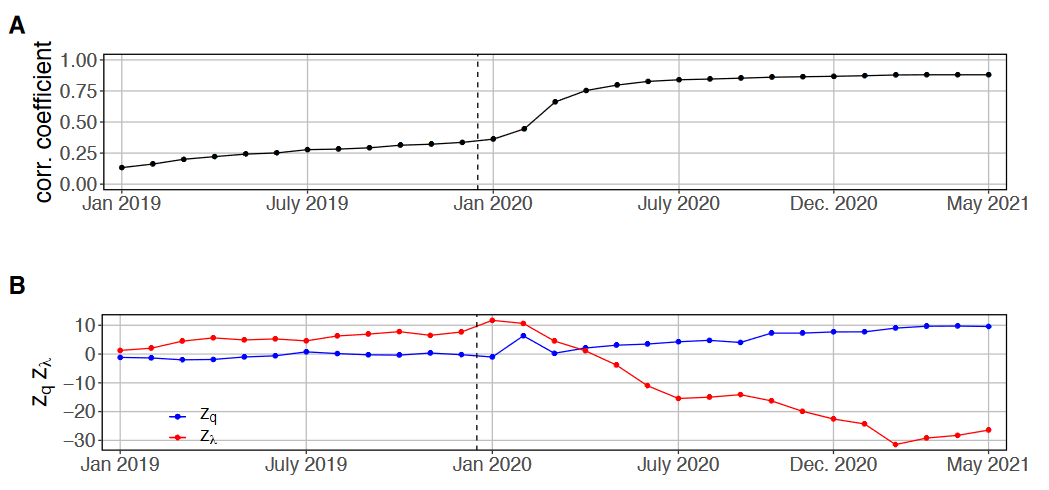
\includegraphics[width=\textwidth]{1_chapter1/figures/Fig6.png} %
\caption{{\bf Convergence of CRR network to non-CRR network.}
{\small In all plots, CRR network is accumulated form Jan. 2019 up to a given month, and the non-CRR network, accumulated from Jan. 2019 to Dec. 2019, serves as the reference network. (A) Pearson's correlation coefficient of (log of) CRR adjacency matrix and non-CRR adjacency matrix. All correlations highly significant according to QAP. (B) Development of $z_q$ (z-value of modularity index Q of CRR network with sampling from non-CRR network for null distribution and communities) and $z_\lambda$ (z-value of largest eigenvalue of CRR network with sampling from non-CRR network for null distribution).}}
\label{fig:NetwConvergenceExtended} 
\end{figure*}

















